% lauritzen_ma_datasheet_conversion.tex
% From datasheet data to the Lauritzen-Ma diode model: theory and conversion rules
% pwr-control template (AAA_template_latex_settings); numbers and figures of the worked examples:
% lm_conversion_calc.py (with the module lm_conversion.py), which writes lm_conversion_values.tex
% Compile: pdflatex lauritzen_ma_datasheet_conversion.tex  (twice, for references)
% Rev. 00 - November 2026 - first issue
\documentclass[10pt,a4paper]{scrartcl}
% ===================== PACKAGES =====================
\usepackage[british]{babel}
\usepackage[tmargin=1in, bmargin=1in, lmargin=0.75in, rmargin=0.75in]{geometry}
\usepackage[dvipsnames,table]{xcolor}  % prima di tikz, listings, ecc.

\usepackage{tikz}
\usepackage{graphicx}
\usepackage{pgfplots}
\pgfplotsset{width=12cm, compat=1.9}
\usepackage{setspace}
\usepackage{chemmacros}
\usepackage{chemfig}
\usepackage{esint}
\usepackage{tabularray}
\usepackage{makeidx}
\usepackage{epstopdf}
\usepackage{amssymb}
\usepackage{mathrsfs}
\usepackage{bm}
\usepackage{amsmath}
\usepackage{enumitem}
\usepackage[english]{varioref}
\usepackage{lipsum}
\usepackage{fancyhdr}
\usepackage{float}
\usepackage{empheq}
\usepackage[framemethod=tikz]{mdframed}
\numberwithin{equation}{section}
\usepackage{eso-pic}
\usepackage{calc}
\usepackage{nccmath}
\usepackage{caption}
\usepackage{subcaption}
\usepackage{gensymb}
\usepackage{amsfonts, amsthm, epsfig, epstopdf, titling, url, array}
\usepackage{tabularx}
\usepackage{makecell}
\usepackage{booktabs}
\usepackage{array}
\usepackage{siunitx}
\sisetup{input-digits=0123456789\pi}
\usepackage[symbol]{footmisc}
\usepackage{multicol}
\usepackage{boondox-cal}
\usepackage{blindtext}
\usepackage{changepage}
\usepackage{nomencl}
\usepackage{hyperref}
\usepackage{xurl}
\usepackage{ragged2e}
\usepackage[version=4]{mhchem}  % ← conflitto di opzioni
\usepackage{longtable}
\usepackage{chemformula}
\usetikzlibrary{arrows.meta,positioning,calc}

% ===================== SI UNITS =====================
\DeclareSIUnit\atm{atm}
\DeclareSIUnit{\var}{var}
\DeclareSIUnit{\pu}{p.u.}


% ===================== MATH OPERATORS =====================
\DeclareMathOperator{\rank}{rank}
\DeclareMathOperator{\atantwo}{atan2}
\DeclareMathOperator{\spn}{span}

% ===================== COMMANDS =====================
\newcommand{\abs}[1]{\left|#1\right|}
\newcommand{\sign}{\text{sign}}
\newcommand{\centered}[1]{\begin{tabular}{@{}l@{}} #1 \end{tabular}}

% ===================== COLORS =====================
\definecolor{mycolor1}{rgb}{0.97, 0.97, 0.97}
\definecolor{mycolor2}{rgb}{0.97, 0.97, 0.97}
\definecolor{tableShade}{gray}{0.9}

% ===================== THEOREM ENVIRONMENTS =====================
\theoremstyle{it}
\newtheorem{defn}{Definition}[section]
\newtheorem{assumption}{Assumption}[section]
\newtheorem{thm}{Theorem}[section]
\newtheorem{lemma}{Lemma}[section]
\newtheorem{corollary}{Corollary}[section]
\theoremstyle{definition}
\newtheorem{example}{Example}[section]

% ===================== CUSTOM ENVIRONMENTS =====================
\newenvironment{myitemize_1}{
	\begin{itemize}[topsep=0pt]
		\setlength{\topsep}{2pt}
		\setlength{\itemsep}{2pt}
		\setlength{\parskip}{2pt}
		\setlength{\parsep}{2pt}
	}{\end{itemize}}

\newmdenv[
innerlinewidth=0.5pt,
roundcorner=4pt,
backgroundcolor=mycolor2,
linecolor=mycolor1,
innerleftmargin=6pt,
innerrightmargin=6pt,
innertopmargin=6pt,
innerbottommargin=6pt
]{mybox}

% ===================== TABLE COLUMN TYPES =====================
\newcolumntype{Y}{>{\hsize=2\hsize}X}
\newcolumntype{Z}{>{\centering\arraybackslash\hsize=0.857\hsize}X}

% ===================== SECTION DEPTH =====================
\setcounter{secnumdepth}{3}
\setcounter{tocdepth}{3}

% ===================== PAGE STYLE =====================
\setlength{\headheight}{20pt}
\setlength{\headsep}{20pt}

\pagestyle{fancy}
\fancypagestyle{firstpage}{\rhead{}}
\fancyhead[L]{\slshape\nouppercase{\leftmark}}
\chead{}
\rhead{\includegraphics[height=0.75cm]{../../AAA_template_latex_settings/pwr-control_logo_doc.png}}
\lfoot{\href{http://www.pwr-control.com}{pwr-control.com}}
\cfoot{-\ \thepage\ -}
\rfoot{\textit{}}
\renewcommand{\headrulewidth}{0.4pt}
\renewcommand{\footrulewidth}{0.4pt}


\geometry{
	a4paper,
	top    = 2.5cm,
	bottom = 3.0cm,
	left   = 2.5cm,
	right  = 2.5cm
}

\hypersetup{
	colorlinks = true,
	urlcolor   = blue,
	linkcolor  = black,
	citecolor  = black
}

\pagenumbering{gobble}
% the document sits four levels below the repository root: logo path of settings.tex corrected here
\rhead{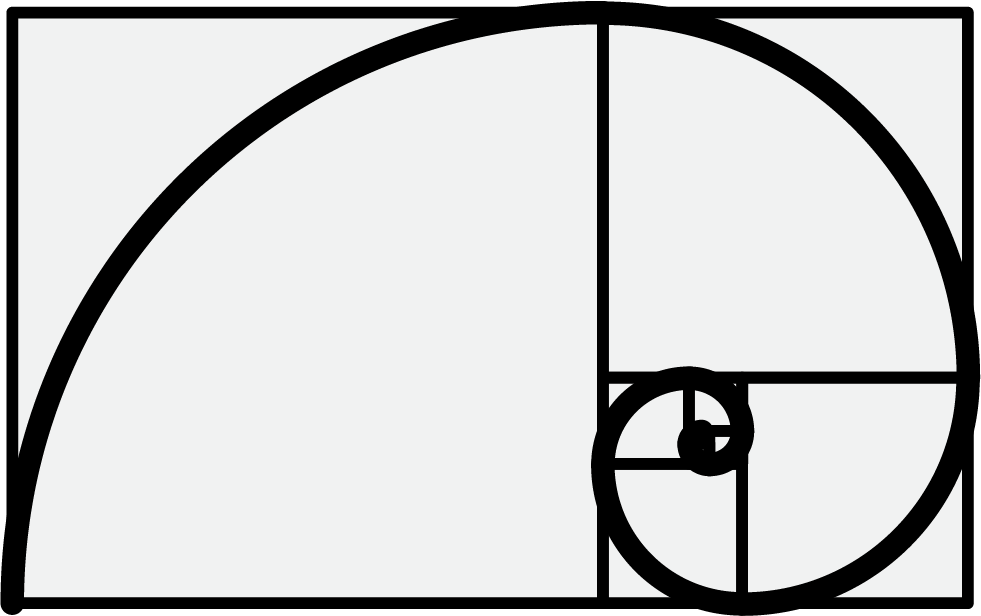
\includegraphics[height=0.75cm]{../../../../AAA_template_latex_settings/pwr-control_logo_doc.png}}
\rfoot{\small Rev.~00}
\geometry{left=2.0cm, right=2.0cm}
\usepackage[european resistors, american inductors]{circuitikz}

\sisetup{per-mode=symbol,range-phrase={\text{--}},range-units=single}
\setlist{nosep}
\setlength{\parindent}{0pt}
\setlength{\parskip}{3pt}
\allowdisplaybreaks
\captionsetup{font=small,labelfont=bf}
\renewcommand{\topfraction}{0.9}
\renewcommand{\bottomfraction}{0.9}
\renewcommand{\textfraction}{0.05}
\renewcommand{\floatpagefraction}{0.8}

% --- numbers of the worked examples (generated by lm_conversion_calc.py) ---
% generated by lm_conversion_calc.py: do not edit by hand
\newcommand{\lmKLine}{1.879}
\newcommand{\lmKTen}{2.303}
\newcommand{\lmKQuarter}{1.386}
\newcommand{\lmKLineHalf}{0.94}
\newcommand{\lmKLineLossPct}{6}
\newcommand{\lmKTenGainPct}{15}
\newcommand{\lmKSpread}{0.92}
\newcommand{\lmTEndTaus}{3.9}
\newcommand{\lmPEndPct}{2}
\newcommand{\lmTailFrac}{0.98}
\newcommand{\lmSofStretchThree}{1.74}
\newcommand{\lmFDefTwo}{13.5}
\newcommand{\lmQDefLoTwo}{17.4}
\newcommand{\lmQDefHiTwo}{23.1}
\newcommand{\lmFDefThree}{5.0}
\newcommand{\lmQDefLoThree}{6.6}
\newcommand{\lmQDefHiThree}{8.8}
\newcommand{\lmFDefFour}{1.8}
\newcommand{\lmQDefLoFour}{2.4}
\newcommand{\lmQDefHiFour}{3.3}
\newcommand{\lmFDefFive}{0.7}
\newcommand{\lmQDefLoFive}{0.9}
\newcommand{\lmQDefHiFive}{1.2}
\newcommand{\lmXLong}{3}
\newcommand{\lmQfracRhoLo}{48}
\newcommand{\lmSofRhoLo}{0.50}
\newcommand{\lmQfracRhoMid}{44}
\newcommand{\lmSofRhoMid}{1.08}
\newcommand{\lmQfracRhoHi}{38}
\newcommand{\lmSofRhoHi}{2.00}
\newcommand{\lmTenthErrTwo}{0.6}
\newcommand{\lmTenthErrFour}{3.1}
\newcommand{\lmRatioLoOne}{0.08}
\newcommand{\lmRatioHiOne}{0.21}
\newcommand{\lmRatioOneHalf}{0.21}
\newcommand{\lmRatioOneOne}{0.17}
\newcommand{\lmRatioOneTwo}{0.12}
\newcommand{\lmRatioOneFour}{0.08}
\newcommand{\lmRatioLoFive}{0.12}
\newcommand{\lmRatioHiFive}{0.36}
\newcommand{\lmRatioFiveHalf}{0.36}
\newcommand{\lmRatioFiveOne}{0.28}
\newcommand{\lmRatioFiveTwo}{0.20}
\newcommand{\lmRatioFiveFour}{0.12}
\newcommand{\lmSensTrrQHalf}{3.0}
\newcommand{\lmSensTrrIHalf}{5.0}
\newcommand{\lmSensTrrAHalf}{2.0}
\newcommand{\lmSensTauQHalf}{0.60}
\newcommand{\lmSensTauIHalf}{0.20}
\newcommand{\lmSensTauAHalf}{0.40}
\newcommand{\lmSensTmQHalf}{3.6}
\newcommand{\lmSensTmIHalf}{6.2}
\newcommand{\lmSensTmAHalf}{2.6}
\newcommand{\lmSensTrrQOne}{2.0}
\newcommand{\lmSensTrrIOne}{3.0}
\newcommand{\lmSensTrrAOne}{1.0}
\newcommand{\lmSensTauQOne}{0.67}
\newcommand{\lmSensTauIOne}{0.33}
\newcommand{\lmSensTauAOne}{0.33}
\newcommand{\lmSensTmQOne}{2.7}
\newcommand{\lmSensTmIOne}{4.3}
\newcommand{\lmSensTmAOne}{1.7}
\newcommand{\lmSensTrrQTwo}{1.5}
\newcommand{\lmSensTrrITwo}{2.0}
\newcommand{\lmSensTrrATwo}{0.5}
\newcommand{\lmSensTauQTwo}{0.75}
\newcommand{\lmSensTauITwo}{0.50}
\newcommand{\lmSensTauATwo}{0.25}
\newcommand{\lmSensTmQTwo}{2.3}
\newcommand{\lmSensTmITwo}{3.5}
\newcommand{\lmSensTmATwo}{1.3}
\newcommand{\lmAIf}{1000}
\newcommand{\lmASlope}{5}
\newcommand{\lmAIrr}{125}
\newcommand{\lmAQrr}{3200}
\newcommand{\lmAVr}{100}
\newcommand{\lmAT}{150}
\newcommand{\lmAVrrm}{4500}
\newcommand{\lmAVrrmKv}{4.5}
\newcommand{\lmAIrrmMa}{50}
\newcommand{\lmATa}{25.0}
\newcommand{\lmAQtri}{1563}
\newcommand{\lmAQtriPct}{49}
\newcommand{\lmAQoverI}{25.6}
\newcommand{\lmATaHalf}{12.5}
\newcommand{\lmATrr}{13.1}
\newcommand{\lmAS}{1.05}
\newcommand{\lmATau}{38.2}
\newcommand{\lmATm}{19.9}
\newcommand{\lmATauL}{38.1}
\newcommand{\lmATmL}{20.0}
\newcommand{\lmARho}{0.34}
\newcommand{\lmATmOverTau}{0.52}
\newcommand{\lmASoftLong}{1.05}
\newcommand{\lmAIrrOverIf}{0.125}
\newcommand{\lmALam}{5.24}
\newcommand{\lmAX}{5.89}
\newcommand{\lmAF}{0.997}
\newcommand{\lmATone}{225}
\newcommand{\lmATzero}{200}
\newcommand{\lmAIter}{7}
\newcommand{\lmATauLErr}{-0.2}
\newcommand{\lmATmLErr}{+0.1}
\newcommand{\lmAIrrBackL}{124.7}
\newcommand{\lmAQrrBackL}{3187}
\newcommand{\lmAIrrBackLErr}{-0.3}
\newcommand{\lmAQrrBackLErr}{-0.4}
\newcommand{\lmAQzero}{7246}
\newcommand{\lmAQzeroPct}{44}
\newcommand{\lmAQstat}{38169}
\newcommand{\lmATrrNinetyEight}{13.4}
\newcommand{\lmATauNinetyEight}{38.4}
\newcommand{\lmATmNinetyEight}{20.5}
\newcommand{\lmAExpIa}{0.99}
\newcommand{\lmAExpQa}{0.98}
\newcommand{\lmAExpIf}{0.01}
\newcommand{\lmAExpQf}{0.02}
\newcommand{\lmANumErr}{6\times10^{-9}}
\newcommand{\lmAIsSecOne}{2.2\times10^{-8}}
\newcommand{\lmARsSecOne}{0.560}
\newcommand{\lmAIsTanOne}{2.8\times10^{-8}}
\newcommand{\lmARsTanOne}{0.564}
\newcommand{\lmAIsSecTwo}{2.5\times10^{-3}}
\newcommand{\lmARsSecTwo}{0.520}
\newcommand{\lmAIsTanTwo}{3.2\times10^{-3}}
\newcommand{\lmARsTanTwo}{0.527}
\newcommand{\lmAVt}{36.46}
\newcommand{\lmAVto}{0.85}
\newcommand{\lmARt}{0.60}
\newcommand{\lmAIone}{500}
\newcommand{\lmAItwo}{1500}
\newcommand{\lmAN}{2}
\newcommand{\lmANmaxSec}{15.0}
\newcommand{\lmANmaxTan}{16.5}
\newcommand{\lmASlopeJct}{0.073}
\newcommand{\lmAVfLine}{1.45}
\newcommand{\lmAVlow}{0.82}
\newcommand{\lmAVlowLine}{0.91}
\newcommand{\lmAVlowDiff}{85}
\newcommand{\lmAVlowOne}{0.87}
\newcommand{\lmAIsStar}{3.8\times10^{-3}}
\newcommand{\lmAIsFactor}{1.52}
\newcommand{\lmAIsOffsetMv}{31}
\newcommand{\lmARr}{90}
\newcommand{\lmADcm}{12}
\newcommand{\lmALdiff}{214}
\newcommand{\lmAWpar}{536}
\newcommand{\lmAWmode}{486}
\newcommand{\lmAWstat}{565}
\newcommand{\lmADoverL}{1.32}
\newcommand{\lmATrrLine}{49.6}
\newcommand{\lmATrrTen}{55.2}
\newcommand{\lmATrrTri}{51.2}
\newcommand{\lmAStretch}{2.21}
\newcommand{\lmASLine}{0.98}
\newcommand{\lmASlopeRatio}{0.52}
\newcommand{\lmAQoverIf}{3.20}
\newcommand{\lmATauIfRatio}{11.9}
\newcommand{\lmAIrrFast}{1914}
\newcommand{\lmAQrrFast}{25069}
\newcommand{\lmAL}{20.0}
\newcommand{\lmAVpk}{291}
\newcommand{\lmAErec}{320}
\newcommand{\lmAOvFactor}{2.91}
\newcommand{\lmASensTauQ}{+0.68}
\newcommand{\lmASensTauI}{-0.35}
\newcommand{\lmASensTauA}{-0.32}
\newcommand{\lmASensTauF}{-0.01}
\newcommand{\lmASensTmQ}{+2.62}
\newcommand{\lmASensTmI}{-4.25}
\newcommand{\lmASensTmA}{+1.62}
\newcommand{\lmASensTmF}{+0.01}
\newcommand{\lmASensTrrQ}{+1.95}
\newcommand{\lmASensTrrI}{-2.91}
\newcommand{\lmASensTrrA}{+0.95}
\newcommand{\lmASensTrrF}{+0.00}
\newcommand{\lmAFiveTau}{-1.6}
\newcommand{\lmAFiveTm}{-19}
\newcommand{\lmAFiveTrr}{-14}
\newcommand{\lmACj}{20}
\newcommand{\lmARsn}{10}
\newcommand{\lmACsn}{470}
\newcommand{\lmACsnUf}{0.47}
\newcommand{\lmARsnCsn}{4.7}
\newcommand{\lmASimSlope}{5.04}
\newcommand{\lmASimSlopeErr}{+0.79}
\newcommand{\lmASimIrrCf}{125.97}
\newcommand{\lmASimIrrDif}{125.84}
\newcommand{\lmASimIrrTerm}{126.12}
\newcommand{\lmASimIrrDifErr}{-0.11}
\newcommand{\lmASimIrrTermErr}{+0.11}
\newcommand{\lmASimQCf}{3192}
\newcommand{\lmASimQDif}{3195}
\newcommand{\lmASimQTerm}{3195}
\newcommand{\lmASimQDifErr}{+0.10}
\newcommand{\lmASimQTermErr}{+0.11}
\newcommand{\lmAQc}{0.31}
\newcommand{\lmAQcPct}{0.01}
\newcommand{\lmASimTrrCf}{49.61}
\newcommand{\lmASimTrr}{49.62}
\newcommand{\lmASimTrrErr}{+0.02}
\newcommand{\lmASimVpk}{289}
\newcommand{\lmASimEd}{310}
\newcommand{\lmASimEr}{15}
\newcommand{\lmASimEsum}{325}
\newcommand{\lmASimEcf}{322}
\newcommand{\lmASimEc}{2.4}
\newcommand{\lmASimEbal}{325}
\newcommand{\lmASimEbalErr}{+0.1}
\newcommand{\lmASimOv}{2.89}
\newcommand{\lmAAwayALo}{0.5}
\newcommand{\lmAAwayIrrALo}{12.5}
\newcommand{\lmAAwayQrrALo}{321}
\newcommand{\lmAAwayXALo}{53.06}
\newcommand{\lmAAwayDsALo}{1604}
\newcommand{\lmAAwayRatioALo}{0.20}
\newcommand{\lmAAwayIcALo}{28.0}
\newcommand{\lmAAwayTauALo}{85.3}
\newcommand{\lmAAwayTmALo}{44.7}
\newcommand{\lmAAwayALoB}{2.5}
\newcommand{\lmAAwayIrrALoB}{62.7}
\newcommand{\lmAAwayQrrALoB}{1607}
\newcommand{\lmAAwayXALoB}{11.14}
\newcommand{\lmAAwayDsALoB}{2599}
\newcommand{\lmAAwayRatioALoB}{0.62}
\newcommand{\lmAAwayIcALoB}{79.7}
\newcommand{\lmAAwayTauALoB}{48.6}
\newcommand{\lmAAwayTmALoB}{25.4}
\newcommand{\lmAAwayARef}{5}
\newcommand{\lmAAwayIrrARef}{125}
\newcommand{\lmAAwayQrrARef}{3200}
\newcommand{\lmAAwayXARef}{5.89}
\newcommand{\lmAAwayDsARef}{3200}
\newcommand{\lmAAwayRatioARef}{1.00}
\newcommand{\lmAAwayIcARef}{125}
\newcommand{\lmAAwayTauARef}{38.2}
\newcommand{\lmAAwayTmARef}{19.9}
\newcommand{\lmAAwayAHiB}{10}
\newcommand{\lmAAwayIrrAHiB}{241}
\newcommand{\lmAAwayQrrAHiB}{6060}
\newcommand{\lmAAwayXAHiB}{3.25}
\newcommand{\lmAAwayDsAHiB}{3940}
\newcommand{\lmAAwayRatioAHiB}{1.54}
\newcommand{\lmAAwayIcAHiB}{196}
\newcommand{\lmAAwayTauAHiB}{30.3}
\newcommand{\lmAAwayTmAHiB}{15.6}
\newcommand{\lmAAwayAHi}{50}
\newcommand{\lmAAwayIrrAHi}{753}
\newcommand{\lmAAwayQrrAHi}{15542}
\newcommand{\lmAAwayXAHi}{0.92}
\newcommand{\lmAAwayDsAHi}{6385}
\newcommand{\lmAAwayRatioAHi}{2.43}
\newcommand{\lmAAwayIcAHi}{558}
\newcommand{\lmAAwayTauAHi}{20.0}
\newcommand{\lmAAwayTmAHi}{8.3}
\newcommand{\lmAAwayFLo}{500}
\newcommand{\lmAAwayIrrFLo}{120}
\newcommand{\lmAAwayQrrFLo}{3030}
\newcommand{\lmAAwayFRef}{1000}
\newcommand{\lmAAwayIrrFRef}{125}
\newcommand{\lmAAwayQrrFRef}{3200}
\newcommand{\lmAAwayFHi}{2000}
\newcommand{\lmAAwayIrrFHi}{125}
\newcommand{\lmAAwayQrrFHi}{3213}
\newcommand{\lmAQexp}{0.30}
\newcommand{\lmAQrangeLo}{0.5}
\newcommand{\lmAQrangeHi}{50}
\newcommand{\lmATauExpCurve}{0.35}
\newcommand{\lmATtwo}{100}
\newcommand{\lmAKt}{0.882}
\newcommand{\lmATauTtwo}{33.7}
\newcommand{\lmATmTtwo}{17.6}
\newcommand{\lmAIrrTtwo}{110}
\newcommand{\lmAQrrTtwo}{2494}
\newcommand{\lmAIrrTtwoPct}{12}
\newcommand{\lmAQrrTtwoPct}{22}
\newcommand{\lmASineLongMs}{10}
\newcommand{\lmASineLongIpk}{15.9}
\newcommand{\lmASineLongWt}{0.012}
\newcommand{\lmASineLongErr}{-0.01}
\newcommand{\lmASineShortMs}{1}
\newcommand{\lmASineShortIpk}{1.59}
\newcommand{\lmASineShortWt}{0.120}
\newcommand{\lmASineShortErr}{-0.80}
\newcommand{\lmALongIrr}{125.3}
\newcommand{\lmBIf}{100}
\newcommand{\lmBSlope}{1000}
\newcommand{\lmBIrr}{80}
\newcommand{\lmBQrr}{12}
\newcommand{\lmBVr}{600}
\newcommand{\lmBT}{125}
\newcommand{\lmBVrrm}{1200}
\newcommand{\lmBVrrmKv}{1.2}
\newcommand{\lmBIrrmMa}{1}
\newcommand{\lmBTa}{80}
\newcommand{\lmBQtri}{3.2}
\newcommand{\lmBQtriPct}{27}
\newcommand{\lmBQoverI}{150}
\newcommand{\lmBTaHalf}{40}
\newcommand{\lmBTrr}{110}
\newcommand{\lmBS}{2.75}
\newcommand{\lmBTau}{278}
\newcommand{\lmBTm}{182}
\newcommand{\lmBTauL}{190}
\newcommand{\lmBTmL}{261}
\newcommand{\lmBRho}{0.40}
\newcommand{\lmBTmOverTau}{0.66}
\newcommand{\lmBSoftLong}{1.31}
\newcommand{\lmBIrrOverIf}{0.80}
\newcommand{\lmBLam}{0.36}
\newcommand{\lmBX}{0.65}
\newcommand{\lmBF}{0.477}
\newcommand{\lmBTone}{180}
\newcommand{\lmBTzero}{100}
\newcommand{\lmBIter}{35}
\newcommand{\lmBTauLErr}{-31.6}
\newcommand{\lmBTmLErr}{+43.4}
\newcommand{\lmBIrrBackL}{42.1}
\newcommand{\lmBQrrBackL}{5.5}
\newcommand{\lmBIrrBackLErr}{-47.3}
\newcommand{\lmBQrrBackLErr}{-54.0}
\newcommand{\lmBQzero}{23.3}
\newcommand{\lmBQzeroPct}{51}
\newcommand{\lmBQstat}{27.8}
\newcommand{\lmBTrrNinetyEight}{112}
\newcommand{\lmBTauNinetyEight}{282}
\newcommand{\lmBTmNinetyEight}{187}
\newcommand{\lmBExpIa}{0.42}
\newcommand{\lmBExpQa}{0.27}
\newcommand{\lmBExpIf}{0.58}
\newcommand{\lmBExpQf}{0.73}
\newcommand{\lmBNumErr}{8\times10^{-9}}
\newcommand{\lmBVt}{34.31}
\newcommand{\lmBN}{1.68}
\newcommand{\lmBRs}{7.2}
\newcommand{\lmBIs}{7.5\times10^{-7}}
\newcommand{\lmBNvt}{57.7}
\newcommand{\lmBIfOne}{25}
\newcommand{\lmBVfOne}{1.18}
\newcommand{\lmBIfTwo}{50}
\newcommand{\lmBVfTwo}{1.40}
\newcommand{\lmBIfThree}{100}
\newcommand{\lmBVfThree}{1.80}
\newcommand{\lmBVto}{1.00}
\newcommand{\lmBRt}{8}
\newcommand{\lmBIsStar}{1.2\times10^{-6}}
\newcommand{\lmBIsFactor}{1.66}
\newcommand{\lmBIsOffsetMv}{29}
\newcommand{\lmBRr}{1.2}
\newcommand{\lmBDcm}{13}
\newcommand{\lmBLdiff}{19}
\newcommand{\lmBWpar}{53}
\newcommand{\lmBWmode}{48}
\newcommand{\lmBWstat}{57}
\newcommand{\lmBDoverL}{1.50}
\newcommand{\lmBTrrLine}{287}
\newcommand{\lmBTrrTen}{333}
\newcommand{\lmBTrrTri}{300}
\newcommand{\lmBStretch}{4.17}
\newcommand{\lmBSLine}{2.58}
\newcommand{\lmBSlopeRatio}{1.37}
\newcommand{\lmBQoverIf}{120}
\newcommand{\lmBTauIfRatio}{2.3}
\newcommand{\lmBIrrFast}{152}
\newcommand{\lmBQrrFast}{16.8}
\newcommand{\lmBL}{0.60}
\newcommand{\lmBVpk}{1036}
\newcommand{\lmBErec}{7.2}
\newcommand{\lmBOvFactor}{1.73}
\newcommand{\lmBSensTauQ}{+0.95}
\newcommand{\lmBSensTauI}{-0.47}
\newcommand{\lmBSensTauA}{-0.05}
\newcommand{\lmBSensTauF}{-0.42}
\newcommand{\lmBSensTmQ}{+1.64}
\newcommand{\lmBSensTmI}{-2.55}
\newcommand{\lmBSensTmA}{+0.64}
\newcommand{\lmBSensTmF}{+0.27}
\newcommand{\lmBSensTrrQ}{+1.36}
\newcommand{\lmBSensTrrI}{-1.73}
\newcommand{\lmBSensTrrA}{+0.36}
\newcommand{\lmBSensTrrF}{+0.00}
\newcommand{\lmBFiveTau}{-2.2}
\newcommand{\lmBFiveTm}{-12}
\newcommand{\lmBFiveTrr}{-8}
\newcommand{\lmBCj}{1}
\newcommand{\lmBRsn}{5.6}
\newcommand{\lmBCsn}{22}
\newcommand{\lmBCsnUf}{0.02}
\newcommand{\lmBRsnCsn}{123}
\newcommand{\lmBSimSlope}{1001}
\newcommand{\lmBSimSlopeErr}{+0.11}
\newcommand{\lmBSimIrrCf}{80.04}
\newcommand{\lmBSimIrrDif}{79.69}
\newcommand{\lmBSimIrrTerm}{81.25}
\newcommand{\lmBSimIrrDifErr}{-0.43}
\newcommand{\lmBSimIrrTermErr}{+1.51}
\newcommand{\lmBSimQCf}{11.83}
\newcommand{\lmBSimQDif}{11.83}
\newcommand{\lmBSimQTerm}{11.86}
\newcommand{\lmBSimQDifErr}{+0.00}
\newcommand{\lmBSimQTermErr}{+0.31}
\newcommand{\lmBQc}{0.040}
\newcommand{\lmBQcPct}{0.33}
\newcommand{\lmBSimTrrCf}{286.6}
\newcommand{\lmBSimTrr}{285.0}
\newcommand{\lmBSimTrrErr}{-0.57}
\newcommand{\lmBSimVpk}{927}
\newcommand{\lmBSimEd}{4.75}
\newcommand{\lmBSimEr}{6.45}
\newcommand{\lmBSimEsum}{11.21}
\newcommand{\lmBSimEcf}{7.20}
\newcommand{\lmBSimEc}{3.96}
\newcommand{\lmBSimEbal}{11.16}
\newcommand{\lmBSimEbalErr}{+0.4}
\newcommand{\lmBSimOv}{1.54}
\newcommand{\lmBAwayALo}{500}
\newcommand{\lmBAwayIrrALo}{56.7}
\newcommand{\lmBAwayQrrALo}{9.5}
\newcommand{\lmBAwayXALo}{1.13}
\newcommand{\lmBAwayARef}{1000}
\newcommand{\lmBAwayIrrARef}{80.0}
\newcommand{\lmBAwayQrrARef}{12.0}
\newcommand{\lmBAwayXARef}{0.65}
\newcommand{\lmBAwayAHi}{2000}
\newcommand{\lmBAwayIrrAHi}{102}
\newcommand{\lmBAwayQrrAHi}{13.9}
\newcommand{\lmBAwayXAHi}{0.36}
\newcommand{\lmBAwayFLo}{50}
\newcommand{\lmBAwayIrrFLo}{51.2}
\newcommand{\lmBAwayQrrFLo}{6.9}
\newcommand{\lmBAwayFRef}{100}
\newcommand{\lmBAwayIrrFRef}{80.0}
\newcommand{\lmBAwayQrrFRef}{12.0}
\newcommand{\lmBAwayFHi}{200}
\newcommand{\lmBAwayIrrFHi}{113}
\newcommand{\lmBAwayQrrFHi}{18.9}
\newcommand{\lmBTtwo}{25}
\newcommand{\lmBIrrTtwo}{55}
\newcommand{\lmBQrrTtwo}{6}
\newcommand{\lmBTrrTtwo}{82}
\newcommand{\lmBTauTtwo}{175}
\newcommand{\lmBTmTtwo}{153}
\newcommand{\lmBTauTtwoPct}{37}
\newcommand{\lmBTmTtwoPct}{16}
\newcommand{\lmBTauExp}{1.6}
\newcommand{\lmBKt}{0.749}
\newcommand{\lmBStepIf}{0.5}
\newcommand{\lmBStepIr}{1}
\newcommand{\lmBStepIrec}{0.25}
\newcommand{\lmBStepIzero}{0.76}
\newcommand{\lmBStepTs}{0}
\newcommand{\lmBStepTrr}{123}
\newcommand{\lmBStepQ}{84}
\newcommand{\lmBStepRatio}{0.5}
\newcommand{\lmBStepIfTwo}{2}
\newcommand{\lmBStepTsTwo}{165}
\newcommand{\lmBStepTrrTwo}{318}
\newcommand{\lmFigRho}{0.35}
\newcommand{\lmFigLam}{2.2}


% --- shorthand ---
\newcommand{\IF}{I_\mathrm{F}}
\newcommand{\IR}{I_\mathrm{R}}
\newcommand{\VR}{V_\mathrm{R}}
\newcommand{\Irr}{I_\mathrm{rr}}
\newcommand{\Qrr}{Q_\mathrm{rr}}
\newcommand{\trr}{t_\mathrm{rr}}
\newcommand{\ta}{t_\mathrm{a}}
\newcommand{\tb}{t_\mathrm{b}}
\newcommand{\ts}{t_\mathrm{s}}
\newcommand{\taurr}{\tau_\mathrm{rr}}
\newcommand{\TM}{T_\mathrm{M}}
\newcommand{\Tone}{T_1}
\newcommand{\qE}{q_\mathrm{E}}
\newcommand{\qM}{q_\mathrm{M}}
\newcommand{\idif}{i_\mathrm{dif}}
\newcommand{\vj}{v_\mathrm{j}}
\newcommand{\IS}{I_\mathrm{S}}
\newcommand{\RS}{R_\mathrm{S}}
\newcommand{\Rr}{R_\mathrm{r}}
\newcommand{\VT}{V_\mathrm{T}}
\newcommand{\VTo}{V_\mathrm{T0}}
\newcommand{\rT}{r_\mathrm{T}}
\newcommand{\Cj}{C_\mathrm{j}}
\newcommand{\Cjo}{C_\mathrm{j0}}
\newcommand{\Csn}{C_\mathrm{sn}}
\newcommand{\Rsn}{R_\mathrm{sn}}
\newcommand{\Vrrm}{V_\mathrm{RRM}}
\newcommand{\Irrm}{I_\mathrm{RRM}}
\newcommand{\Vrm}{V_\mathrm{RM}}
\newcommand{\Tj}{T_\mathrm{j}}
\newcommand{\diff}{\mathrm{d}}
\newcommand{\us}{\si{\micro\second}}
\newcommand{\Aus}{\si{\ampere\per\micro\second}}
\newcommand{\uC}{\si{\micro\coulomb}}

% =============================================================
%  DOCUMENT DATA (title page: AAA_template_latex_settings/titlepage.tex)
% =============================================================
\newcommand{\DocCategory}{Technical Note}
\newcommand{\DocField}{Power Electronics and Control Systems}
\newcommand{\DocTitle}{%
	{\fontsize{20}{24}\selectfont\bfseries From Datasheet Data} \\[16pt]
	{\fontsize{16}{20}\selectfont\bfseries to the Lauritzen--Ma Diode Model}
}
\newcommand{\DocSubtitle}{Theory of the two-charge model of the reverse recovery, direct and inverse relations with the datasheet quantities, limits of the conversion}
\newcommand{\DocAuthor}{Davide Bagnara}
\newcommand{\DocRevision}{00}
\newcommand{\DocDate}{November 2026}
\newcommand{\DocAbstract}{%
The Lauritzen--Ma model describes the reverse recovery of a power diode with two charges and two time constants, the carrier lifetime $\tau$ and the diffusion transit time $\TM$. A datasheet does not give them: it gives the peak reverse recovery current, the recovered charge and the recovery time at one test condition. This note derives the relations between the two descriptions in general form, from the equations of the model. The turn-off on a current ramp is solved exactly for any length of the ramp, and the peak reverse current is given in closed form with the Lambert function; the usual long-ramp formulas and the abrupt-commutation estimates are its two limits. The inverse problem, from the datasheet point to $\tau$ and $\TM$, becomes a fixed-point iteration that always converges and has the long-ramp closed form as its first step; a criterion written with the data alone, the ratio of the peak reverse current to the forward current, says when the closed form is enough. The note also covers the definitions of the recovery time and of the softness, the sensitivity of the parameters to the data, the parameters of the conduction and of the blocking state, the energy and the peak voltage of an inductive commutation, and what the model cannot reproduce: it is linear until the junction blocks, so on a long ramp its recovered charge is proportional to the slope, and it meets a datasheet curve at one point only. Two worked examples with assumed datasheets, a rectifier diode on a long ramp and a fast diode on a short ramp, are checked against a simulated commutation cell; the companion Python scripts reproduce every number and figure.
}
\newcommand{\RevisionHistory}{%
	00 & November 2026 & First issue. & \DocAuthor \\
}
\newcommand{\MetaLabelA}{Project Repository}
\newcommand{\MetaValueAUrl}{https://github.com/pwr-control/repositories-documentation.git}
\newcommand{\MetaValueALabel}{repositories-documentation.git}
\newcommand{\MetaLabelB}{Calculation}
\newcommand{\MetaValueB}{Python 3 / NumPy, SciPy (\texttt{lm\_conversion\_calc.py})}

\begin{document}
% =============================================================
%  pwr-control LaTeX template - FRONTESPIZIO
%
%  Da richiamare come prima istruzione dopo \begin{document}:
%      \input{../../AAA_template_latex_settings/titlepage}
%
%  Il documento deve definire prima di \begin{document}:
%      \DocCategory   categoria del documento
%      \DocField      area tecnica
%      \DocTitle      titolo (una o due righe)
%      \DocSubtitle   sottotitolo
%      \DocAuthor     autore/i, separati da virgola
%      \DocRevision   numero di revisione corrente (es. 00)
%      \DocDate       data della revisione corrente
%      \DocAbstract   abstract
%      \RevisionHistory  righe della tabella di revisione, nel formato
%                        Rev. & Date & Description & Authors \\
%      \MetaLabelA \MetaValueAUrl \MetaValueALabel
%      \MetaLabelB \MetaValueB
% =============================================================

\providecommand{\DocCategory}{Technical Research Report}
\providecommand{\DocField}{Power Electronics and Control Systems}
\providecommand{\DocSubtitle}{}
\providecommand{\DocRevision}{00}
\providecommand{\DocAbstract}{}
\providecommand{\RevisionHistory}{%
	\DocRevision & \DocDate & First issue. & \DocAuthor \\
}

\titlepage

% ---- Intestazione centrata ----
\begin{center}
	{\Large\scshape \DocCategory}\\[8pt]
	{\large\scshape \DocField}
\end{center}

\vspace{30pt plus 4pt minus 14pt}
\noindent\rule{\linewidth}{0.8pt}

% ---- Titolo ----
\begin{center}
	\DocTitle
\end{center}

\vspace{4pt}
\noindent\rule{\linewidth}{2.2pt}

% ---- Sottotitolo ----
\begin{center}
	\begin{onehalfspace}
		{\large\itshape \DocSubtitle}
	\end{onehalfspace}
\end{center}

% ---- Authors / Revision / Date ----
\vspace{30pt plus 4pt minus 14pt}

\noindent
\begin{minipage}[t]{0.46\linewidth}
	\raggedright
	\textbf{Authors:}\\[2pt]
	\DocAuthor
\end{minipage}%
\hfill
\begin{minipage}[t]{0.22\linewidth}
	\centering
	\textbf{Revision:}\\[2pt]
	\DocRevision
\end{minipage}%
\hfill
\begin{minipage}[t]{0.30\linewidth}
	\raggedleft
	\textbf{Date:}\\[2pt]
	\DocDate
\end{minipage}

\vspace{10pt}
\noindent\rule{\linewidth}{0.8pt}

% ---- Abstract ----
\vspace{24pt plus 4pt minus 12pt}

\begin{center}
	\begin{minipage}{0.88\linewidth}
		\footnotesize
		\begin{onehalfspace}
			\textbf{Abstract:} \DocAbstract
		\end{onehalfspace}
	\end{minipage}
\end{center}

\vfill

% ---- Revision history ----
\begin{center}
	\begin{minipage}{0.96\linewidth}
		\centering
		{\footnotesize\scshape Revision history}\\[6pt]
		{\footnotesize
			\begin{tabular}{@{}cl>{\raggedright\arraybackslash}p{0.36\linewidth}>{\raggedright\arraybackslash}p{0.28\linewidth}@{}}
				\toprule
				\textbf{Rev.} & \textbf{Date} & \textbf{Description} & \textbf{Authors} \\
				\midrule
				\RevisionHistory
				\bottomrule
			\end{tabular}}
	\end{minipage}
\end{center}

\vspace{18pt plus 4pt minus 10pt}

% ---- Metadati in fondo ----
\noindent
\begin{tabular}{@{} r @{\quad} l @{}}
	\textsc{\MetaLabelA:} & {\href{\MetaValueAUrl}{\MetaValueALabel}} \\[3pt]
	\textsc{\MetaLabelB:} & {\MetaValueB}       \\[3pt]
\end{tabular}

% =============================================================
%  Fine frontespizio
% =============================================================
\newpage
\pagenumbering{arabic}
\setcounter{page}{1}

\tableofcontents
\newpage

%=====================================================================
\section{Scope and results}
\label{sec:scope}
A circuit simulation of a diode turn-off needs a diode model that stores charge. The model of Lauritzen and Ma \cite{lauritzen1991} is the simplest one that gives a soft recovery. It has one state variable, the charge stored in the middle of the diode, and two parameters for the recovery: the carrier lifetime $\tau$ and the diffusion transit time $\TM$. It is the diode with charge dynamics of several circuit simulators (Sec.~\ref{sec:others}) and of the component \texttt{diode\_rr} of the pwr-control library.

A datasheet does not give $\tau$ and $\TM$. It gives what a test on a current ramp shows: the peak reverse recovery current, the recovered charge, the recovery time, each with its own definition and at one test condition. This note derives the relations between the two descriptions, in both directions:
\begin{itemize}
\item from the model to the datasheet quantities (Secs.~\ref{sec:ramp} and~\ref{sec:direct}): what a given pair $\tau$, $\TM$ does on a current ramp of any length, and in other test circuits;
\item from the datasheet to the model (Secs.~\ref{sec:inverse} and~\ref{sec:static}): which data fix which parameter, when a closed form is enough, and how the tolerance of the data moves the parameters;
\item what the model cannot reproduce, whatever the parameters (Sec.~\ref{sec:limits}).
\end{itemize}
All relations follow from the equations of the model (Sec.~\ref{sec:model}); nothing is fitted. Section~\ref{sec:examples} applies them to two diodes and checks the result in a simulated commutation cell, and Sec.~\ref{sec:procedure} collects the procedure. The data of the two diodes are assumed: round values typical of a rectifier diode and of a fast diode, not the data of a product.

Two notes of this repository treat neighbouring subjects: the charge-control model of the diode from the continuity equation, in \texttt{research/power\_semiconductor\_devices/diode/charge\_control\_model}, and the recovered charge of a rectifier diode at the slow slope of a transformer-fed bridge, in \texttt{research/diode-stack} (Sec.~6).

\subsection*{The results in short}
\begin{enumerate}
\item On a current ramp of slope $a$ the model gives a triangle followed by an exponential tail (Fig.~\ref{fig:waveform}). The tail has the time constant $\taurr = \tau\TM/(\tau+\TM)$, and the recovered charge is $\Qrr = \Irr^2/(2a) + \Irr\,\taurr$ for any length of the ramp. So the datasheet point gives $\taurr = \Qrr/\Irr - \Irr/(2a)$ with no approximation, \eqref{eq:taurr}.
\item The peak reverse current is $\Irr = a\,(\tau-\taurr)\,\bigl(1-e^{-\Tone/\tau}\bigr)$, where $\Tone = (\IF+\Irr)/a$ is the length of the ramp from the forward current $\IF$ to the peak, \eqref{eq:peak}. It has a closed form with the Lambert function, \eqref{eq:lambert}. On a long ramp, $\Tone \geq 5\tau$, the bracket is one: the peak no longer depends on the forward current and the conversion is the closed form $\tau = \taurr + \Irr/a$, $\TM = \tau\,\taurr\,a/\Irr$, \eqref{eq:longinv}.
\item For any ramp the exact $\tau$ is the limit of the iteration $\tau \leftarrow \taurr + (\Irr/a)\big/\bigl(1-e^{-\Tone/\tau}\bigr)$, which starts from the closed form and always converges, \eqref{eq:iter}. The closed form alone is within \SI{1}{\percent} when the datasheet has $\Irr/\IF$ below about \num{0.1} to \num{0.2}, depending on the softness (Table~\ref{tab:valid}); for a fast diode tested with $\Irr$ close to $\IF$ it is wrong by tens of percent.
\item The two parameters have separate roles. On a long ramp $\tau$ sets the size of the recovery, $\Qrr = a\,(\tau^2-\taurr^2)/2$, and the ratio $\TM/\tau$ sets its shape: the softness is $s = 2\TM/\tau$, \eqref{eq:softlong}.
\item The recovery time depends on its definition. For the exponential tail the fall time is $\tb = \kappa\,\taurr$ with $\kappa = \lmKLine$ for the straight line through \SI{90}{\percent} and \SI{25}{\percent} of the peak, \num{\lmKTen} for the instant at \SI{10}{\percent}, and 2 for the triangle of equal charge (Table~\ref{tab:kappa}).
\item The lifetime is a robust result of the conversion and the transit time is a fragile one: a peak current higher by \SI{5}{\percent} at the same charge moves $\tau$ by about \SI{2}{\percent} and $\TM$ by \SIrange{10}{20}{\percent} (Sec.~\ref{sec:sens}).
\item Until the junction blocks the model is linear. Its $\Irr$ and $\Qrr$ are therefore homogeneous of degree one in the pair $(a, \IF)$: the exponents against the slope and against the forward current add up to one, \eqref{eq:euler}. On a long ramp both grow in proportion to the slope. A datasheet curve of the charge against the slope is much flatter, so one parameter set meets it at one point: the parameters have to be extracted at the slope of the application (Sec.~\ref{sec:limits}).
\item In an inductive commutation the energy dissipated after the current zero is $\VR\,\Qrr$, plus $\Csn\VR^2/2$ if an RC snubber sits across the diode, and without snubber the peak reverse voltage is $\VR\,(1+2/s)$ (Sec.~\ref{sec:energy}).
\end{enumerate}

%=====================================================================
\section{Nomenclature}
\label{sec:nomenclature}
\begin{center}\small
\begin{tabular}{@{}>{$}l<{$}>{\raggedright\arraybackslash}p{6.5cm}>{$}l<{$}>{\raggedright\arraybackslash}p{6.0cm}@{}}
\toprule
i,\ v & current and voltage of the diode, positive in the forward direction & \tau & carrier lifetime (parameter of the model) \\
\IF & forward current before the turn-off & \TM & diffusion transit time (parameter of the model) \\
a & rate of fall of the current, $a = -\diff i/\diff t > 0$ & \taurr & time constant of the recovery tail, $\tau\TM/(\tau+\TM)$ \\
\VR & reverse voltage applied by the circuit & \rho & $\taurr/\tau = \TM/(\tau+\TM)$ \\
\Irr & peak reverse recovery current (IEC: $I_\mathrm{rrm}$; also $I_\mathrm{RM}$) & \lambda & normalised forward current, $\IF/(a\tau)$ \\
\Qrr & recovered charge (IEC: $Q_\mathrm{r}$; also $Q_\mathrm{S}$) & y & normalised peak current, $\Irr/(a\tau)$ \\
\ta & time from the current zero to the peak, $\Irr/a$ & \Tone,\ x & length of the ramp to the peak, $(\IF+\Irr)/a$, and $x = \Tone/\tau$ \\
\tb & fall time, from the peak to the end of the recovery & s & softness, $2\taurr/\ta$ \\
\trr & reverse recovery time, $\ta+\tb$ & \kappa & fall time of the tail in units of $\taurr$ \\
\qE,\ \qM & edge charge and middle charge of the model & \IS,\ n & saturation current and emission coefficient \\
\idif & diffusion current, $(\qE-\qM)/\TM$ & \VT & thermal voltage, $kT/q$ \\
\vj & junction voltage & \RS,\ \Rr & series resistance, leakage resistance \\
\VTo,\ \rT & threshold voltage and slope resistance of the datasheet & \Cj,\ \Cjo & junction capacitance, its value at zero voltage \\
\Vrrm,\ \Irrm & repetitive peak reverse voltage, reverse current at $\Vrrm$ & L & commutation inductance, $a = \VR/L$ \\
\bottomrule
\end{tabular}
\end{center}
Recovery quantities are positive numbers: $\Irr$ is the magnitude of the peak of the reverse current and $\Qrr$ the magnitude of the charge.

%=====================================================================
\section{The quantities of the datasheet}
\label{sec:datasheet}
\subsection{Reverse recovery}
\label{sec:rrdata}
In the recovery test the diode first carries the forward current $\IF$. The circuit then forces the current down at a constant rate $a = -\diff i/\diff t$, through zero and into the reverse direction (Fig.~\ref{fig:waveform}a). The reverse current rises to the peak $\Irr$, which it reaches at the time $\ta$ after the current zero; the diode then takes up the reverse voltage $\VR$ and the current falls back to zero in the time $\tb$. The datasheet gives some of the following quantities, with the test conditions $\IF$, $a$, $\VR$ and the junction temperature.
\begin{itemize}
\item \emph{Peak reverse recovery current} $\Irr$ ($I_\mathrm{rrm}$ in IEC~60747-2 \cite{iec60747}, 3.3.10; $I_\mathrm{RM}$ or $I_\mathrm{RR}$ in many datasheets).
\item \emph{Recovered charge} $\Qrr$ ($Q_\mathrm{r}$ in \cite{iec60747}, 3.5.5; also $Q_\mathrm{rr}$, $Q_\mathrm{S}$): the integral of the reverse current from the current zero. The standard ends the integral at the instant at which the current has fallen to \SI{\lmPEndPct}{\percent} of the peak, and notes that the charge includes components due to both carrier storage and depletion-layer capacitance (3.5.5, Note~2).
\item \emph{Reverse recovery time} $\trr = \ta + \tb$ (\cite{iec60747}, 3.5.2), from the current zero to the end of the recovery. The current approaches zero asymptotically, so the end needs a convention. The standard draws a straight line through two points A and B of the falling current and takes the instant at which the line reaches zero; A is often specified at \SI{90}{\percent} and B at \SI{25}{\percent} of the peak (3.5.2, Note~5). The same construction is in \cite{an6481}, Sec.~2.1. Other documents take the instant at which the current has fallen to a fraction of the peak: \SI{10}{\percent} in the documentation of the simulators \cite{mathworks,plecs}, a fraction $k$, usually \num{0.25}, in \cite{an5028}. The standard names the two parts of $\trr$ rise time and fall time (3.5.3, 3.5.4).
\item \emph{Softness}: the ratio $\tb/\ta$ (\cite{an6481}, Sec.~2.1; \cite{an5028}), or a ratio of the two slopes of the reverse current. A diode is called soft when the current comes back slowly from the peak and snappy when it comes back abruptly.
\end{itemize}
Rectifier diodes for line frequency usually come with the maximum $\Qrr$ and $\Irr$ at the maximum junction temperature and at a slope of a few \Aus, and with curves of the two quantities against the slope. Fast diodes come with typical $\Irr$, $\Qrr$ and $\trr$ at two temperatures and at hundreds or thousands of \Aus, with curves against the forward current and the slope.

\begin{figure}[htb]
\centering
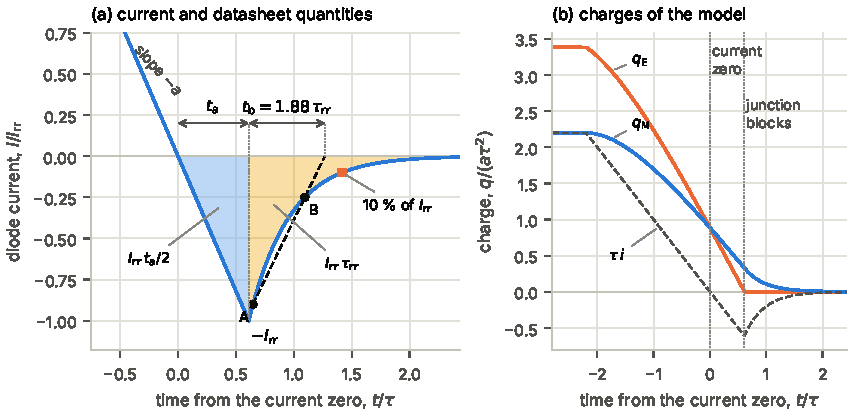
\includegraphics[width=\textwidth]{figures/fig_waveform.pdf}
\caption{Turn-off of the model on a current ramp ($\rho = \lmFigRho$, $\IF/(a\tau) = \lmFigLam$). (a) Current and datasheet quantities: the triangle of charge $\Irr\ta/2$, the tail of charge $\Irr\taurr$, the straight line through the points A (\SI{90}{\percent}) and B (\SI{25}{\percent}) that defines $\tb$, and the point at \SI{10}{\percent}. (b) The two charges of the model and, dashed, $\tau i$: the middle charge $\qM$ follows the current with a delay, the edge charge $\qE$ reaches zero after the current, and at that instant the junction blocks.}
\label{fig:waveform}
\end{figure}

\subsection{Forward characteristic}
For a rectifier diode the datasheet gives the forward voltage at one current and a straight-line approximation of the characteristic at the maximum temperature,
\begin{equation}
v \approx \VTo + \rT\, i ,
\label{eq:line}
\end{equation}
with the threshold voltage $\VTo$ and the slope resistance $\rT$. The line crosses the real characteristic at two currents, which the datasheet states or which are implied by the range of validity of the line. For a fast diode the datasheet gives the forward voltage at the rated current and a curve at two temperatures.

\subsection{Blocking state}
The datasheet gives the reverse current $\Irrm$ at the repetitive peak reverse voltage $\Vrrm$ and at the maximum temperature, as a maximum. A junction capacitance is given for small and fast diodes, at a low reverse voltage; for large rectifier diodes it is usually not given.

%=====================================================================
\section{The model}
\label{sec:model}
\subsection{Equations}
The model describes the charge carriers stored in the lightly doped middle region of the diode (the base) with two charges (Fig.~\ref{fig:model}a). The \emph{middle charge} $\qM$ is the charge stored in the base. The \emph{edge charge} $\qE$ stands for the carrier concentration at the edges of the base, next to the junction, and is tied to the junction voltage. Carriers diffuse from the edge to the middle, and this diffusion is the current of the diode:
\begin{align}
\idif &= \frac{\qE - \qM}{\TM} , \label{eq:idif}\\
\frac{\diff \qM}{\diff t} &= \idif - \frac{\qM}{\tau} , \label{eq:qm}\\
\qE &= (\tau+\TM)\,\IS\,\bigl(e^{\vj/(n\VT)} - 1\bigr) . \label{eq:qe}
\end{align}
Equation \eqref{eq:qm} is the balance of the middle charge: the diffusion current feeds it and recombination removes it with the lifetime $\tau$. Equation \eqref{eq:idif} says that the current is driven by the difference of the two charges and that $\TM$ is the time the carriers take to diffuse into the base. Equation \eqref{eq:qe} is the junction law. The complete diode adds the junction capacitance, a leakage resistance and a series resistance:
\begin{equation}
i = \idif + \Cj(\vj)\,\frac{\diff \vj}{\diff t} + \frac{\vj}{\Rr} , \qquad v = \vj + \RS\, i .
\label{eq:terminal}
\end{equation}
The model has one state for the stored charge, $\qM$, because $\qE$ is an algebraic function of the junction voltage. The equations are the lumped-charge description of Linvill \cite{linvill1958} applied to the base of a power diode \cite{lauritzen1991}; Appendix~\ref{app:lumped} shows where they come from and what $\TM$ is in terms of the width of the base.

In \eqref{eq:qe} the factor in front of the bracket is written so that $\IS$ is the saturation current of the static characteristic, as in \cite{mathworks}. Some implementations, the library component \texttt{diode\_rr} among them, write $\qE = \tau\,\IS^{*}\,(e^{\vj/(n\VT)}-1)$. The two forms are the same model with
\begin{equation}
\IS^{*} = \IS\,\frac{\tau+\TM}{\tau} .
\label{eq:isstar}
\end{equation}

\begin{figure}[htb]
\centering
\begin{circuitikz}[scale=0.9, transform shape]
\ctikzset{bipoles/length=1.0cm}
% (a) the model
\node[anchor=west] at (-0.6,2.6) {(a)};
\draw (0,0) node[left]{A} to[short, o-] (0.3,0) to[R, l=$\RS$] (2.3,0) coordinate (J);
\draw (J) -- (2.3,1.5) to[american controlled current source, l={$\idif$}] (5.3,1.5) -- (5.3,0) coordinate (K);
\draw (J) to[C, l=$\Cj(\vj)$, *-*] (K);
\draw (J) -- (2.3,-1.5) to[R, l=$\Rr$] (5.3,-1.5) -- (K);
\draw (K) to[short, -o] (6.2,0) node[right]{K};
\draw[-{Latex[length=2mm]}] (0.4,0.42) -- (0.95,0.42) node[midway, above]{$i$};
\node at (2.55,-2.0) {$+$}; \node at (3.8,-2.0) {$\vj$}; \node at (5.05,-2.0) {$-$};
% (b) the commutation cell
\begin{scope}[xshift=8.8cm, yshift=-1.6cm]
\node[anchor=west] at (-0.9,4.2) {(b)};
\draw (0,0) to[american voltage source, invert, l=$\VR$] (0,3.2) to[closing switch, l={$t=0$}] (1.7,3.2) to[L, l=$L$] (3.4,3.2) -- (6.4,3.2);
\draw (3.4,0) to[D*, l=D, *-*] (3.4,3.2);
\draw (4.9,3.2) to[R, l=$\Rsn$, *-] (4.9,1.6) to[C, l=$\Csn$, -*] (4.9,0);
\draw (6.4,3.2) to[american current source, l=$\IF$] (6.4,0);
\draw (0,0) -- (6.4,0);
\draw[-{Latex[length=2mm]}] (3.05,0.35) -- (3.05,0.95) node[midway, left]{$i$};
\end{scope}
\end{circuitikz}
\caption{(a) Equivalent circuit of the model: the diffusion current $\idif = (\qE-\qM)/\TM$, with $\qM$ from \eqref{eq:qm} and $\qE$ from \eqref{eq:qe}, in parallel with the junction capacitance and the leakage resistance, and in series with $\RS$. (b) Commutation cell: the diode carries the current $\IF$ of the load; at $t=0$ the switch applies the voltage $\VR$ in reverse through the inductance $L$, and the diode current falls with the slope $a = \VR/L$. An RC snubber may sit across the diode.}
\label{fig:model}
\end{figure}

\subsection{Static characteristic}
In the steady state $\diff\qM/\diff t = 0$, so \eqref{eq:idif} and \eqref{eq:qm} give
\begin{equation}
\qM = \tau\, i , \qquad \qE = (\tau+\TM)\, i , \qquad i = \IS\,\bigl(e^{\vj/(n\VT)}-1\bigr) .
\label{eq:static}
\end{equation}
At rest the model is the ordinary diode equation with a series resistance, and the base holds the charge $\tau\,i$. The parameters $\IS$, $n$ and $\RS$ shape the forward characteristic and have no part in the recovery, as long as the forward voltage is small against the voltages of the circuit.

\subsection{Two regimes and two time constants}
\label{sec:regimes}
The diode works in one of two regimes.

\emph{Conducting junction} ($\qE > 0$). The junction voltage is a forward voltage of about a volt, whatever the sign of the current. The circuit sets the current, and the charges follow it: with $\idif = i$,
\begin{equation}
\frac{\diff \qM}{\diff t} = i - \frac{\qM}{\tau} , \qquad \qE = \qM + \TM\, i .
\label{eq:conducting}
\end{equation}
The first relation is the classical charge-control equation with the time constant $\tau$. The second says that the edge charge is the middle charge plus a part proportional to the current. A reverse current can flow in this regime: it only needs $\qM > \TM\,|i|$.

\emph{Blocked junction} ($\qE = 0$). The edge charge cannot go below zero: in \eqref{eq:qe} a reverse voltage brings the bracket to $-1$ and $\qE$ to $-(\tau+\TM)\IS$, which is nothing on the scale of the stored charge. With $\qE = 0$,
\begin{equation}
\idif = -\frac{\qM}{\TM} , \qquad \frac{\diff\qM}{\diff t} = -\qM\Bigl(\frac1\TM + \frac1\tau\Bigr) = -\frac{\qM}{\taurr} , \qquad \taurr = \frac{\tau\,\TM}{\tau+\TM} .
\label{eq:blocked}
\end{equation}
The diode is now a current source that decays with the time constant $\taurr$, whatever the circuit does; the circuit sets the voltage. The charge left in the base leaves by diffusion to the edges (the reverse current) and by recombination, and the two rates add. The tail time constant is always shorter than both $\tau$ and $\TM$. The ratio
\begin{equation}
\rho = \frac{\taurr}{\tau} = \frac{\TM}{\tau+\TM}
\label{eq:rho}
\end{equation}
is used below as the shape parameter of the model, with $0 < \rho < 1$.

Seen from the current, the edge charge of the conducting junction is a filtered copy of the current. From \eqref{eq:conducting}, in the Laplace domain,
\begin{equation}
\frac{\qE(s)}{i(s)} = (\tau+\TM)\,\frac{1+s\,\taurr}{1+s\,\tau} .
\label{eq:filter}
\end{equation}
This is a lag network. For a current that changes slowly on the scale of $\tau$ it is a pure delay of $\tau-\taurr$: the edge charge is $(\tau+\TM)$ times the current of $\tau-\taurr$ earlier. The junction blocks when $\qE$ crosses zero, so on a slow ramp it blocks $\tau-\taurr$ after the current zero, when the reverse current has grown to $a\,(\tau-\taurr)$. This is the whole reverse recovery of the model in one line; Section~\ref{sec:ramp} makes it exact.

\subsection{Parameters}
\begin{table}[htb]
\centering\small
\caption{Parameters of the model and the datasheet data that fix them.}
\label{tab:params}
\begin{tabular}{@{}llp{6.4cm}c@{}}
\toprule
Parameter & Role & Datasheet data & Section \\
\midrule
$\tau$, $\TM$ & reverse recovery & two of $\Irr$, $\Qrr$, $\trr$ at a stated slope and forward current & \ref{sec:inverse} \\
$\IS$, $n$, $\RS$ & forward characteristic & $\VTo$ and $\rT$, or points of the forward curve & \ref{sec:forward} \\
$\Rr$ & leakage in the blocking state & reverse current at a reverse voltage & \ref{sec:blocking} \\
$\Cjo$, $V_\mathrm{j}$, $m$ & junction capacitance & capacitance at a reverse voltage, or an estimate & \ref{sec:blocking} \\
\bottomrule
\end{tabular}
\end{table}
The four groups of Table~\ref{tab:params} are independent: each can be converted without the others. The recovery parameters are the subject of the next three sections.

%=====================================================================
\section{Turn-off on a current ramp}
\label{sec:ramp}
\subsection{Assumptions}
The diode is in the steady state with the forward current $\IF$. From $t = 0$ the circuit forces the current down at the constant rate $a$:
\begin{equation}
i(t) = \IF - a\,t .
\label{eq:ramp}
\end{equation}
In the commutation cell of Fig.~\ref{fig:model}b the slope is $a = \VR/L$. The circuit imposes the ramp as long as the junction conducts, because the junction voltage is small against $\VR$. The junction capacitance and the leakage are left out in this section; Section~\ref{sec:cell} shows their effect on the two examples.

\subsection{Charges during the ramp}
With \eqref{eq:ramp} and the initial value $\qM(0) = \tau\IF$, the solution of \eqref{eq:conducting} is
\begin{align}
\qM(t) &= \tau\,(\IF - a\,t) + a\,\tau^2\,\bigl(1 - e^{-t/\tau}\bigr) , \label{eq:qmramp}\\
\qE(t) &= (\tau+\TM)\,(\IF - a\,t) + a\,\tau^2\,\bigl(1 - e^{-t/\tau}\bigr) . \label{eq:qeramp}
\end{align}
The first term of \eqref{eq:qmramp} is the charge the diode would hold if it followed the current without delay. The second term is the delay: charge that is still in the base because recombination needs time. At the current zero, $t_0 = \IF/a$, the first term vanishes and the two charges are equal:
\begin{equation}
\qM(t_0) = a\,\tau^2\,\bigl(1 - e^{-\IF/(a\tau)}\bigr) .
\label{eq:qzero}
\end{equation}
The charge present at the current zero is not the static charge $\tau\IF$. On a ramp that lasts several lifetimes it is $a\,\tau^2$, whatever the forward current: the charge that was there at the start has recombined on the way, and what is left is what the last few lifetimes of the ramp have fed. Figure~\ref{fig:waveform}b shows the two charges.

\subsection{Peak reverse current}
The junction blocks at the instant $\Tone$ at which $\qE$ reaches zero. The current at that instant is the peak, $i(\Tone) = -\Irr$, so $\Tone = (\IF+\Irr)/a$. Equation \eqref{eq:qeramp} with $\qE(\Tone) = 0$, and with $\tau^2/(\tau+\TM) = \tau - \taurr$, gives
\begin{equation}
\Irr = a\,(\tau-\taurr)\,\bigl(1 - e^{-\Tone/\tau}\bigr) , \qquad \Tone = \frac{\IF+\Irr}{a} .
\label{eq:peak}
\end{equation}
This is an implicit equation for $\Irr$, because $\Tone$ contains it. The time from the current zero to the peak is $\ta = \Irr/a$. Up to the peak the diode voltage is still a small forward voltage, although the current is already reversed.

\subsection{Tail and recovered charge}
After $\Tone$ the junction is blocked and \eqref{eq:blocked} holds, with $\qM(\Tone) = \TM\Irr$:
\begin{equation}
i(t) = -\Irr\,e^{-(t-\Tone)/\taurr} , \qquad t \geq \Tone .
\label{eq:tail}
\end{equation}
The reverse current is a triangle of base $\ta$ followed by an exponential, with a corner at the peak. Its integral is the recovered charge
\begin{equation}
\Qrr = \frac{\Irr\,\ta}{2} + \Irr\,\taurr = \frac{\Irr^2}{2a} + \Irr\,\taurr .
\label{eq:qrr}
\end{equation}
Equation \eqref{eq:qrr} holds for any length of the ramp: it only uses the shape of the waveform.

\subsection{Normalised form and closed-form solution}
\label{sec:norm}
With the normalised quantities
\begin{equation}
y = \frac{\Irr}{a\,\tau} , \qquad \lambda = \frac{\IF}{a\,\tau} , \qquad \rho = \frac{\taurr}{\tau} ,
\label{eq:normdef}
\end{equation}
equations \eqref{eq:peak} and \eqref{eq:qrr} become
\begin{equation}
y = (1-\rho)\,\bigl(1 - e^{-(\lambda+y)}\bigr) , \qquad \frac{\Qrr}{a\,\tau^2} = \frac{y^2}{2} + \rho\,y .
\label{eq:norm}
\end{equation}
The normalised recovery depends on two numbers only: the shape parameter $\rho$, and $\lambda$, which is the time the ramp takes to reach the current zero counted in lifetimes. The first of \eqref{eq:norm} has the solution
\begin{equation}
y = (1-\rho) + W_0\!\left(-(1-\rho)\,e^{-(\lambda+1-\rho)}\right) ,
\label{eq:lambert}
\end{equation}
where $W_0$ is the principal branch of the Lambert function, the inverse of $w \mapsto w\,e^{w}$ (Appendix~\ref{app:lambert}). The Lambert term is negative: it is what the finite length of the ramp takes away from the long-ramp value $1-\rho$. Figure~\ref{fig:map} shows the result.

\begin{figure}[htb]
\centering
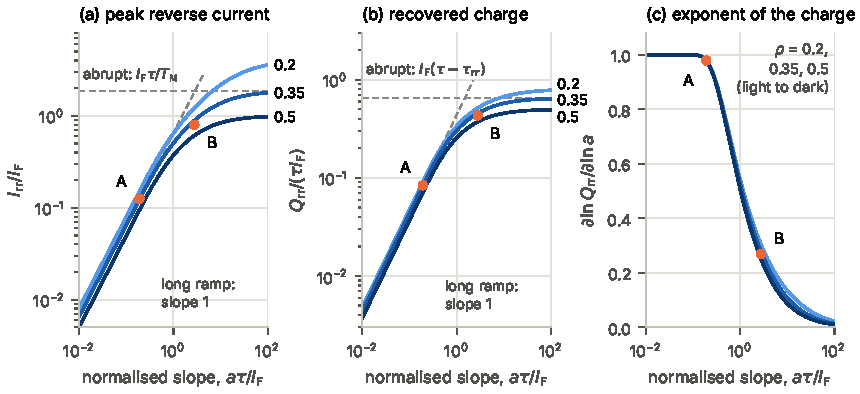
\includegraphics[width=\textwidth]{figures/fig_map.pdf}
\caption{Recovery of the model against the normalised slope $a\tau/\IF = 1/\lambda$, for three values of $\rho$. (a) Peak reverse current and (b) recovered charge, with the two asymptotes of the middle curve: the long ramp \eqref{eq:long}, with slope one, and the abrupt commutation \eqref{eq:abrupt}, a constant. (c) Local exponent of the charge against the slope, \eqref{eq:exponents}. The points A and B are the two worked examples of Sec.~\ref{sec:examples} at their datasheet conditions.}
\label{fig:map}
\end{figure}

\subsection{Long ramp and abrupt commutation}
\label{sec:limitsramp}
\emph{Long ramp} ($\lambda \to \infty$). The exponential of \eqref{eq:peak} vanishes:
\begin{equation}
\Irr = a\,(\tau - \taurr) = \frac{a\,\tau^2}{\tau+\TM} , \qquad \ta = \tau - \taurr , \qquad \Qrr = \frac{a}{2}\,\bigl(\tau^2 - \taurr^2\bigr) .
\label{eq:long}
\end{equation}
Peak and charge are proportional to the slope and do not depend on the forward current. The time to the peak is a constant of the diode: it is the delay $\tau - \taurr$ of \eqref{eq:filter}.

The factor $1 - e^{-x}$ of \eqref{eq:peak}, with $x = \Tone/\tau$, says how long a ramp has to be. Table~\ref{tab:long} gives what is missing to the long-ramp values. A ramp is long, for the purpose of a conversion, when it lasts five lifetimes from the forward current to the peak; with three lifetimes the long-ramp formulas are off by \SI{\lmFDefThree}{\percent} on the peak and by up to \SI{\lmQDefHiThree}{\percent} on the charge.

\begin{table}[htb]
\centering\small
\caption{Peak current and charge of the model on a ramp of finite length, relative to the long-ramp values \eqref{eq:long}. The range of the charge is for $\rho$ from 0.5 to 0.1.}
\label{tab:long}
\begin{tabular}{@{}lcccc@{}}
\toprule
Length of the ramp, $x = \Tone/\tau$ & 2 & 3 & 4 & 5 \\
\midrule
$\Irr$ below the long-ramp value by & \SI{\lmFDefTwo}{\percent} & \SI{\lmFDefThree}{\percent} & \SI{\lmFDefFour}{\percent} & \SI{\lmFDefFive}{\percent} \\
$\Qrr$ below the long-ramp value by & \SIrange{\lmQDefLoTwo}{\lmQDefHiTwo}{\percent} & \SIrange{\lmQDefLoThree}{\lmQDefHiThree}{\percent} & \SIrange{\lmQDefLoFour}{\lmQDefHiFour}{\percent} & \SIrange{\lmQDefLoFive}{\lmQDefHiFive}{\percent} \\
\bottomrule
\end{tabular}
\end{table}

\emph{Abrupt commutation} ($\lambda \to 0$). The ramp is so fast that nothing recombines before the junction blocks. The middle charge is still $\tau\IF$ when the edge charge is pulled to zero, and \eqref{eq:blocked} gives
\begin{equation}
\Irr \to \IF\,\frac{\tau}{\TM} , \qquad \Qrr \to \IF\,(\tau - \taurr) = \IF\,\frac{\tau^2}{\tau+\TM} .
\label{eq:abrupt}
\end{equation}
Peak and charge are proportional to the forward current and no longer depend on the slope. These are the largest values the model can give for a forward current.

\subsection{Charge balance}
Of the charge present at the current zero, \eqref{eq:qzero}, only a part comes out of the terminals. The rest recombines during the recovery. On a long ramp, from \eqref{eq:long},
\begin{equation}
\frac{\Qrr}{\qM(t_0)} = \frac{1-\rho^2}{2} .
\label{eq:fraction}
\end{equation}
Less than half of the charge at the current zero is recovered: \SI{\lmQfracRhoLo}{\percent} for $\rho = 0.2$, \SI{\lmQfracRhoMid}{\percent} for $\rho = 0.35$, \SI{\lmQfracRhoHi}{\percent} for $\rho = 0.5$. In an abrupt commutation the recovered part of the static charge $\tau\IF$ is $1-\rho$, from \eqref{eq:abrupt}. The recovered charge of a datasheet is therefore never the stored charge of the diode, and the lifetime cannot be read as $\Qrr/\IF$ (Sec.~\ref{sec:others}).

\subsection{Dependence on the slope and on the forward current}
\label{sec:exponents}
While the junction conducts, the equations \eqref{eq:conducting} are linear, and the blocking condition $\qE = 0$ does not change if the current and the charges are all multiplied by the same factor. So if the slope and the forward current are both multiplied by $k$, the whole waveform is multiplied by $k$: $\Irr$ and $\Qrr$ are homogeneous functions of degree one of the pair $(a, \IF)$, as \eqref{eq:normdef} and \eqref{eq:norm} show. By Euler's theorem on homogeneous functions
\begin{equation}
\frac{\partial \ln \Irr}{\partial \ln a} + \frac{\partial \ln \Irr}{\partial \ln \IF} = 1 , \qquad
\frac{\partial \ln \Qrr}{\partial \ln a} + \frac{\partial \ln \Qrr}{\partial \ln \IF} = 1 .
\label{eq:euler}
\end{equation}
In a log-log plot the slope of a curve against $a$ and the slope of the curve against $\IF$ add up to one, at every point. The exponents against the slope follow from \eqref{eq:norm} (Appendix~\ref{app:exponents}):
\begin{equation}
\frac{\partial \ln \Irr}{\partial \ln a} = 1 - \frac{\lambda\,(1-\rho-y)}{y\,(\rho+y)} , \qquad
\frac{\partial \ln \Qrr}{\partial \ln a} = 1 - \frac{\lambda\,(1-\rho-y)}{y^2/2+\rho\,y} .
\label{eq:exponents}
\end{equation}
On a long ramp $y = 1-\rho$ and both exponents are one: the recovery is proportional to the slope and blind to the forward current. In an abrupt commutation both are zero and the recovery is proportional to the forward current. Figure~\ref{fig:map}c shows the passage from one to the other, which takes about two decades of slope around $a\tau = \IF$.

%=====================================================================
\section{From the model to the datasheet quantities}
\label{sec:direct}
\subsection{Recovery time and softness}
\label{sec:trr}
With the exponential tail \eqref{eq:tail}, every convention for the end of the recovery gives a fall time proportional to the tail time constant:
\begin{equation}
\tb = \kappa\,\taurr , \qquad \trr = \ta + \kappa\,\taurr .
\label{eq:trr}
\end{equation}
For a straight line through the points at the fractions $p_\mathrm{A}$ and $p_\mathrm{B}$ of the peak,
\begin{equation}
\kappa = \ln\frac{1}{p_\mathrm{A}} + \frac{p_\mathrm{A}}{p_\mathrm{A}-p_\mathrm{B}}\,\ln\frac{p_\mathrm{A}}{p_\mathrm{B}} ,
\label{eq:kappaline}
\end{equation}
and for the instant at which the current has fallen to the fraction $p$ of the peak, $\kappa = \ln(1/p)$. Table~\ref{tab:kappa} gives the values. Between the conventions the fall time of the same waveform differs by up to \num{\lmKSpread} tail time constants, so a recovery time cannot be converted without its convention.

\begin{table}[htb]
\centering\small
\caption{Conventions for the end of the recovery and fall time of an exponential tail, $\tb = \kappa\,\taurr$.}
\label{tab:kappa}
\begin{tabular}{@{}lcl@{}}
\toprule
Convention & $\kappa$ & Used in \\
\midrule
straight line through \SI{90}{\percent} and \SI{25}{\percent} of the peak, extended to zero & \lmKLine & \cite{iec60747}, 3.5.2 Note~5; \cite{an6481}, Sec.~2.1 \\
current fallen to \SI{25}{\percent} of the peak & \lmKQuarter & \cite{an5028} ($k$ usually \num{0.25}) \\
current fallen to \SI{10}{\percent} of the peak & \lmKTen & \cite{mathworks}, \cite{plecs} \\
triangle with the same charge as the tail & 2 & this note, \eqref{eq:soft} \\
\bottomrule
\end{tabular}
\end{table}

This note measures the softness with the ratio of the charge of the tail to the charge of the triangle,
\begin{equation}
s = \frac{\Irr\,\taurr}{\Irr\,\ta/2} = \frac{2\,\taurr}{\ta} .
\label{eq:soft}
\end{equation}
It is the ratio $\tb/\ta$ for the triangle of equal charge ($\kappa = 2$); the ratio $\tb/\ta$ of the straight-line convention is \num{\lmKLineHalf}\,$s$. From \eqref{eq:peak}, $\ta = (\tau-\taurr)\,(1-e^{-x})$, so
\begin{equation}
s = \frac{2\,\TM}{\tau}\,\frac{1}{1-e^{-x}} \quad\longrightarrow\quad s = \frac{2\,\TM}{\tau} \quad \text{on a long ramp.}
\label{eq:softlong}
\end{equation}
On a long ramp the softness of the model is a constant of the diode: twice the ratio of its two parameters. It does not depend on the slope, on the forward current or on the voltage. On a short ramp the softness is larger, because the triangle shrinks and the tail time constant does not. The documentation \cite{mathworks} uses the stretch factor $\trr\,a/\Irr$ with the \SI{10}{\percent} convention, which is $1 + (\ln 10/2)\,s$; its typical value of 3 corresponds to $s = \lmSofStretchThree$.

\subsection{Recovered charge}
Equation \eqref{eq:qrr} is the integral of the whole reverse current. If the integral ends where the current has fallen to the fraction $p$ of the peak, as in the standard with $p = \SI{\lmPEndPct}{\percent}$, the fraction $p$ of the tail charge is cut:
\begin{equation}
Q_\mathrm{r} = \frac{\Irr\,\ta}{2} + (1-p)\,\Irr\,\taurr .
\label{eq:qrp}
\end{equation}
The integral then lasts $\ln(1/p) = \lmTEndTaus$ tail time constants. The difference from \eqref{eq:qrr} is below the tolerance of any datasheet value; it is used in Sec.~\ref{sec:cell} to compare a simulation with the closed form on equal terms. A second difference is the charge of the junction capacitance, which a measured value includes and \eqref{eq:qrr} does not (Sec.~\ref{sec:blocking}).

The estimate $\Qrr \approx \Irr\,\trr/2$ is exact with the equal-charge convention. With the straight-line convention it misses \SI{\lmKLineLossPct}{\percent} of the tail charge, and with the \SI{10}{\percent} convention it adds \SI{\lmKTenGainPct}{\percent} to it.

\subsection{Peak voltage and energy in an inductive commutation}
\label{sec:energy}
In the cell of Fig.~\ref{fig:model}b without snubber and without capacitance, the diode voltage stays near zero up to the peak of the reverse current. In the tail the diode imposes the current \eqref{eq:tail} on the inductance, and its reverse voltage is
\begin{equation}
v_\mathrm{R}(t) = \VR + \frac{L\,\Irr}{\taurr}\,e^{-(t-\Tone)/\taurr} .
\end{equation}
The peak is at the blocking instant. With $L = \VR/a$,
\begin{equation}
\Vrm = \VR + \frac{L\,\Irr}{\taurr} = \VR\,\Bigl(1 + \frac{\ta}{\taurr}\Bigr) = \VR\,\Bigl(1 + \frac{2}{s}\Bigr) .
\label{eq:vrm}
\end{equation}
The peak voltage depends on the softness only: a diode with $s = 1$ triples the applied voltage, one with $s = 4$ adds half of it. The energy dissipated in the diode during the tail is
\begin{equation}
E = \int v_\mathrm{R}\,|i|\,\diff t = \VR\,\Irr\,\taurr + \frac{L\,\Irr^2}{2} = \VR\,\Qrr .
\label{eq:erec}
\end{equation}
The first form is in \cite{mathworks}; the second follows with $L = \VR/a$ and \eqref{eq:qrr}. It contains the energy that the inductance holds at the peak.

In the model the voltage steps from zero to $\Vrm$ at the blocking instant. A real circuit has capacitance across the diode, which rounds the step and can lower the peak; a snubber does it on purpose. With an RC snubber across the diode the balance of the energy from the current zero to the end of the transient is
\begin{equation}
E_\mathrm{D} + E_\mathrm{R} = \VR\,\Qrr + \frac{\Csn\,\VR^2}{2} ,
\label{eq:ebal}
\end{equation}
where $E_\mathrm{D}$ is the energy dissipated in the diode and $E_\mathrm{R}$ the energy dissipated in the snubber resistor. The source delivers $\VR$ times the charge of the diode and of the snubber capacitor, and the capacitor keeps $\Csn\VR^2/2$. The sum does not depend on the snubber resistor: the snubber moves a part of $\VR\,\Qrr$ from the diode to the resistor and adds the charging loss of its capacitor.

\subsection{Other test circuits}
\label{sec:othertests}
\emph{Resistive commutation.} Small and fast diodes are often tested with a step: the forward current $\IF$ is reversed abruptly and the circuit limits the reverse current to $\IR$. While the junction conducts, the reverse current stays at $\IR$; this is the storage phase. Equation \eqref{eq:conducting} with $i = -\IR$ gives $\qM(t) = -\tau\IR + \tau\,(\IF+\IR)\,e^{-t/\tau}$, and $\qE = \qM - \TM\IR$ reaches zero at the storage time
\begin{equation}
\ts = \tau\,\ln\!\left[\Bigl(1+\frac{\IF}{\IR}\Bigr)\,\frac{\tau}{\tau+\TM}\right] \qquad \text{if} \quad \frac{\IF}{\IR} > \frac{\TM}{\tau} .
\label{eq:ts}
\end{equation}
After the storage time the current decays from $\IR$ with the time constant $\taurr$. If $\IF/\IR \leq \TM/\tau$ there is no storage phase: the junction blocks at once, the reverse current starts from $\IF\,\tau/\TM$, which is the abrupt limit \eqref{eq:abrupt}, and decays from there. With $\TM \to 0$ equation \eqref{eq:ts} becomes $\ts = \tau\ln(1+\IF/\IR)$, the storage time of the charge-control model with one charge.

\emph{Half-sine pulse.} The standard has a half-sinusoidal and a rectangular measuring method (\cite{iec60747}, 6.3.5). For a sinusoidal current $\hat I\sin\omega t$ that has lasted long on the scale of $\tau$, \eqref{eq:filter} gives the edge charge as a sinusoid delayed by the phase $\arctan\omega\tau - \arctan\omega\taurr$. The junction blocks at this phase after the current zero, so
\begin{equation}
\Irr = \hat I\,\sin\bigl(\arctan\omega\tau - \arctan\omega\taurr\bigr) .
\label{eq:sine}
\end{equation}
For $\omega\tau \ll 1$ this is $\omega\hat I\,(\tau-\taurr)$: the long-ramp result \eqref{eq:long} with the slope $a = \omega\hat I$ of the sinusoid at its zero.

%=====================================================================
\section{From the datasheet to the model}
\label{sec:inverse}
\subsection{From the peak current and the charge}
\label{sec:invpq}
The datasheet gives $\Irr$ and $\Qrr$ at a slope $a$ and a forward current $\IF$. The conversion has four steps.
\begin{enumerate}
\item Time to the peak: $\ta = \Irr/a$.
\item Tail time constant, from \eqref{eq:qrr}:
\begin{equation}
\taurr = \frac{\Qrr}{\Irr} - \frac{\Irr}{2a} .
\label{eq:taurr}
\end{equation}
This step is exact for any ramp; the same relation is Eq.~(2) of \cite{an6481}. It needs $\Qrr > \Irr^2/(2a)$: the charge has to be larger than the triangle. A pair of data that violates the condition has no tail and cannot be represented by the model.
\item Lifetime, from \eqref{eq:peak} written as
\begin{equation}
\tau = \taurr + \frac{\ta}{1 - e^{-\Tone/\tau}} , \qquad \Tone = \frac{\IF+\Irr}{a} .
\label{eq:iter}
\end{equation}
Equation \eqref{eq:iter} is used as an iteration: the right-hand side is evaluated with the current value of $\tau$, starting from $\tau = \taurr + \ta$. The iteration converges for any data, to the only solution, and at each step the error shrinks by a factor smaller than $\Irr/(\IF+\Irr)$ (Appendix~\ref{app:contraction}).
\item Transit time, from the definition of $\taurr$:
\begin{equation}
\TM = \frac{\tau\,\taurr}{\tau - \taurr} .
\label{eq:tm}
\end{equation}
\end{enumerate}
On a long ramp the exponential of \eqref{eq:iter} is zero and the starting value is already the result:
\begin{equation}
\tau = \taurr + \ta = \frac{\Qrr}{\Irr} + \frac{\Irr}{2a} , \qquad \TM = \frac{\tau\,\taurr}{\ta} .
\label{eq:longinv}
\end{equation}
This is the closed form found in the notes on the model; it does not contain the forward current.

\subsection{When the closed form is enough}
\label{sec:valid}
The closed form \eqref{eq:longinv} is exact for $x = \Tone/\tau \to \infty$. Whether a datasheet point is on a long ramp can be seen from the data alone, because $x$ follows from the ratio $\Irr/\IF$ and from the softness $s = 2\taurr/\ta$:
\begin{equation}
x = \frac{1 + \IF/\Irr}{s/2 + 1/(1-e^{-x})} \;\approx\; \frac{1 + \IF/\Irr}{1 + s/2} .
\label{eq:xdata}
\end{equation}
A set obtained with the closed form from a point that is not on a long ramp is not the diode of the datasheet: put back on the test ramp it returns a lower peak and a lower charge. Figure~\ref{fig:inversion} shows this error and Table~\ref{tab:valid} gives the limits. When the peak reverse current of the datasheet is below a tenth of the forward current, the set of the closed form returns the peak and the charge within \SI{\lmTenthErrTwo}{\percent} for a softness up to 2 and within \SI{\lmTenthErrFour}{\percent} for a softness of 4. For a fast diode tested with a peak reverse current close to the forward current it is wrong by tens of percent, and \eqref{eq:iter} has to be used. The iteration costs nothing, so the simple rule is to iterate always.

\begin{table}[htb]
\centering\small
\caption{Largest ratio $\Irr/\IF$ of the datasheet point for which the set of the closed form \eqref{eq:longinv} returns the peak current of the datasheet within the stated error.}
\label{tab:valid}
\begin{tabular}{@{}lcccc@{}}
\toprule
Softness of the datasheet point, $s = 2\taurr/\ta$ & 0.5 & 1 & 2 & 4 \\
\midrule
$\Irr$ returned within \SI{1}{\percent} for $\Irr/\IF$ below & \lmRatioOneHalf & \lmRatioOneOne & \lmRatioOneTwo & \lmRatioOneFour \\
$\Irr$ returned within \SI{5}{\percent} for $\Irr/\IF$ below & \lmRatioFiveHalf & \lmRatioFiveOne & \lmRatioFiveTwo & \lmRatioFiveFour \\
\bottomrule
\end{tabular}
\end{table}

\begin{figure}[htb]
\centering
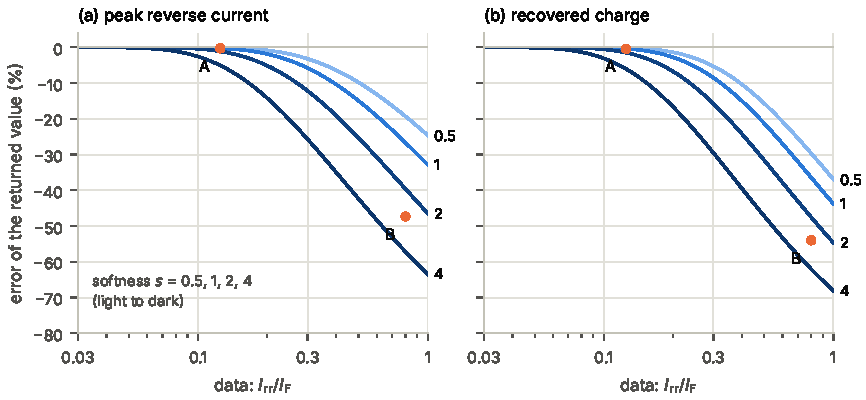
\includegraphics[width=\textwidth]{figures/fig_inversion.pdf}
\caption{Error of the long-ramp closed form \eqref{eq:longinv}: the set it gives is put back on the test ramp and (a) its peak current and (b) its charge are compared with the data, against the ratio $\Irr/\IF$ of the datasheet point and for four values of the softness. A and B are the two worked examples.}
\label{fig:inversion}
\end{figure}

\subsection{From other pairs of data}
\label{sec:pairs}
The recovery has two parameters, so two independent data at one test condition are needed. With pairs other than $(\Irr, \Qrr)$ the first two steps of Sec.~\ref{sec:invpq} change and the other two stay.

\emph{Peak current and recovery time.} From \eqref{eq:trr}, with the $\kappa$ of the convention of the datasheet,
\begin{equation}
\taurr = \frac{\trr - \Irr/a}{\kappa} .
\label{eq:fromtrr}
\end{equation}
It needs $\trr > \Irr/a$.

\emph{Charge and recovery time.} Eliminating $\taurr$ between \eqref{eq:qrr} and \eqref{eq:trr} gives a quadratic equation for the peak current, $(1-\kappa/2)\,\Irr^2 - a\,\trr\,\Irr + \kappa\,a\,\Qrr = 0$, with the solution
\begin{equation}
\Irr = \frac{a}{2-\kappa}\left[\trr - \sqrt{\trr^2 - \frac{2\,\kappa\,(2-\kappa)\,\Qrr}{a}}\,\right] \quad (\kappa \neq 2) , \qquad \Irr = \frac{2\,\Qrr}{\trr} \quad (\kappa = 2) .
\label{eq:fromqt}
\end{equation}
This is the root with $\Irr < a\,\trr$; it exists when $\Qrr < a\,\trr^2/2$. Then \eqref{eq:fromtrr} gives $\taurr$.

\emph{One datum only.} With the charge alone, or the recovery time alone, the shape has to be assumed. With an assumed softness $s$, from \eqref{eq:qrr} and \eqref{eq:soft},
\begin{equation}
\Irr = \sqrt{\frac{2\,a\,\Qrr}{1+s}} , \qquad \taurr = \frac{s\,\Irr}{2a} .
\label{eq:fromq}
\end{equation}

\emph{Three data.} When the datasheet gives $\Irr$, $\Qrr$ and $\trr$, the three are consistent with an exponential tail if $\Qrr = \Irr\,[\ta/2 + (\trr-\ta)/\kappa]$. Usually they are not exactly, because a real tail is not an exponential. The pair $(\Irr, \Qrr)$ is then the better choice: the peak and the charge are what the circuit feels, and they do not depend on a convention. The recovery time is a check.

\subsection{Sensitivity to the data}
\label{sec:sens}
Datasheet values have tolerances, and the two values of a pair are often maxima that do not belong to the same device. On a long ramp the logarithmic derivatives of \eqref{eq:taurr} and \eqref{eq:longinv} are
\begin{equation}
\begin{aligned}
\frac{\diff\taurr}{\taurr} &= \frac{1+s}{s}\,\frac{\diff\Qrr}{\Qrr} - \frac{2+s}{s}\,\frac{\diff\Irr}{\Irr} + \frac{1}{s}\,\frac{\diff a}{a} , \\
\frac{\diff\tau}{\tau} &= \frac{1+s}{2+s}\,\frac{\diff\Qrr}{\Qrr} - \frac{s}{2+s}\,\frac{\diff\Irr}{\Irr} - \frac{1}{2+s}\,\frac{\diff a}{a} , \\
\frac{\diff\TM}{\TM} &= \frac{\diff\tau}{\tau} + \frac{\diff\taurr}{\taurr} - \frac{\diff\Irr}{\Irr} + \frac{\diff a}{a} .
\end{aligned}
\label{eq:sens}
\end{equation}

\begin{table}[htb]
\centering\small
\caption{Relative change of the parameters for a relative change of one datum of one percent, on a long ramp, from \eqref{eq:sens}.}
\label{tab:sens}
\begin{tabular}{@{}lccccccccc@{}}
\toprule
 & \multicolumn{3}{c}{$s = 0.5$} & \multicolumn{3}{c}{$s = 1$} & \multicolumn{3}{c}{$s = 2$} \\
\cmidrule(lr){2-4}\cmidrule(lr){5-7}\cmidrule(l){8-10}
Datum & $\tau$ & $\taurr$ & $\TM$ & $\tau$ & $\taurr$ & $\TM$ & $\tau$ & $\taurr$ & $\TM$ \\
\midrule
$\Qrr$ & $+\lmSensTauQHalf$ & $+\lmSensTrrQHalf$ & $+\lmSensTmQHalf$ & $+\lmSensTauQOne$ & $+\lmSensTrrQOne$ & $+\lmSensTmQOne$ & $+\lmSensTauQTwo$ & $+\lmSensTrrQTwo$ & $+\lmSensTmQTwo$ \\
$\Irr$ & $-\lmSensTauIHalf$ & $-\lmSensTrrIHalf$ & $-\lmSensTmIHalf$ & $-\lmSensTauIOne$ & $-\lmSensTrrIOne$ & $-\lmSensTmIOne$ & $-\lmSensTauITwo$ & $-\lmSensTrrITwo$ & $-\lmSensTmITwo$ \\
$a$ & $-\lmSensTauAHalf$ & $+\lmSensTrrAHalf$ & $+\lmSensTmAHalf$ & $-\lmSensTauAOne$ & $+\lmSensTrrAOne$ & $+\lmSensTmAOne$ & $-\lmSensTauATwo$ & $+\lmSensTrrATwo$ & $+\lmSensTmATwo$ \\
\bottomrule
\end{tabular}
\end{table}

Table~\ref{tab:sens} reads as follows. The lifetime is a robust result: all its coefficients are below one. The tail time constant and the transit time are fragile, the more so the snappier the diode: $\taurr$ is the difference of two terms of similar size, $\Qrr/\Irr$ and $\ta/2$, and for $s = 0.5$ a peak current higher by \SI{1}{\percent} lowers $\TM$ by \SI{\lmSensTmIHalf}{\percent}. The softness of the model, $2\TM/\tau$, is therefore known only roughly from a pair of datasheet values. When the peak voltage or the damping of a commutation depend on it, the transit time has to be checked on a measured waveform, or the calculation repeated with $\TM$ at the two ends of its range.

\subsection{Which data to convert}
\label{sec:which}
\begin{itemize}
\item \emph{Maximum or typical.} A set converted from the maximum $\Qrr$ and $\Irr$ is the device with the largest charge. For the spread between the devices of a series connection a second device with a lower charge is needed. If only its charge is known, the softness is kept: on a long ramp \eqref{eq:long} gives $\Qrr \propto \tau^2$ and $\Irr \propto \tau$ at a fixed ratio $\TM/\tau$, so a device with the charge $\Qrr'$ at the same slope has
\begin{equation}
\tau' = \tau\,\sqrt{\Qrr'/\Qrr} , \qquad \TM' = \TM\,\sqrt{\Qrr'/\Qrr} .
\label{eq:scale}
\end{equation}
\item \emph{Temperature.} A set holds at the temperature of its data. Lifetime and recovered charge grow with the temperature [M] \cite{lutz}, so the data of the highest working temperature give the largest recovery. If the datasheet gives the charge at a second temperature only as a ratio or a curve, \eqref{eq:scale} applies.
\item \emph{Test point.} If the datasheet gives the recovery at several slopes, the point to convert is the one nearest to the slope of the application. Section~\ref{sec:limits} explains why.
\end{itemize}

%=====================================================================
\section{Conduction and blocking parameters}
\label{sec:static}
\subsection{Forward characteristic}
\label{sec:forward}
From \eqref{eq:static} and \eqref{eq:terminal} the static characteristic of the model is
\begin{equation}
v = n\,\VT\,\ln\Bigl(1 + \frac{i}{\IS}\Bigr) + \RS\, i .
\label{eq:vf}
\end{equation}
It has three parameters. The straight line \eqref{eq:line} has two numbers, so one parameter has to be chosen, and it is the emission coefficient $n$. The line gives no information on it: three points on a straight line, fitted with \eqref{eq:vf}, return $n = 0$.

\emph{Choice of $n$.} At its working currents a power diode has the base in high injection. The carrier concentration at the edges of the base then grows with $e^{\vj/(2\VT)}$, where $\vj$ is the sum of the voltages of the two junctions (Appendix~\ref{app:lumped}), and since $\qE$ stands for that concentration the model wants $n = 2$. The value $n = 1$ belongs to low injection. A fit to a measured curve can return other values, because the three parameters then also absorb what the model does not have, for example a resistance of the base that depends on the current.

\emph{Tangent fit.} The model is made tangent to the line at one current $I_0$, for example the forward current of the application:
\begin{equation}
\RS = \rT - \frac{n\,\VT}{I_0} , \qquad \IS = \frac{I_0}{e^{(\VTo + n\VT)/(n\VT)} - 1} .
\label{eq:tangent}
\end{equation}
The first relation matches the slopes, because the junction has the incremental resistance $n\VT/I_0$; the second matches the voltages, because the junction voltage at $I_0$ is then $\VTo + n\VT$. Everywhere else the model lies below the line, by $n\VT\,(x - 1 - \ln x)$ with $x = i/I_0$.

\emph{Secant fit.} The model crosses the line at the two currents $I_1$ and $I_2$ at which the line crosses the real characteristic:
\begin{equation}
\RS = \rT - \frac{n\,\VT\,\ln(I_2/I_1)}{I_2 - I_1} , \qquad \IS = \frac{I_1}{e^{[\VTo + (\rT-\RS)\,I_1]/(n\VT)} - 1} .
\label{eq:secant}
\end{equation}
The first relation neglects $\IS$ against $I_1$. Both fits need $\RS \geq 0$, which limits the emission coefficient to $n \leq \rT I_0/\VT$ for the tangent and to $n \leq \rT\,(I_2-I_1)/(\VT\ln(I_2/I_1))$ for the secant.

\emph{Points of a curve.} For $i \gg \IS$ equation \eqref{eq:vf} is linear in the three unknowns $n\VT$, $n\VT\ln\IS$ and $\RS$:
\begin{equation}
v_k = n\VT\,\ln i_k - n\VT\,\ln\IS + \RS\, i_k .
\label{eq:points}
\end{equation}
Three points of the forward curve give the three parameters by a linear system, and more points by least squares. The points should span the working range of the current.

\emph{Implementations with $\tau\,\IS^{*}$.} A saturation current found from the static characteristic is the $\IS$ of \eqref{eq:qe}. An implementation that writes the junction law with $\tau\,\IS^{*}$ needs $\IS^{*} = \IS\,(\tau+\TM)/\tau$, \eqref{eq:isstar}. If the factor is forgotten the forward voltage of the model is too high by $n\VT\ln[(\tau+\TM)/\tau]$, a few tens of millivolts.

\subsection{Blocking state and junction capacitance}
\label{sec:blocking}
\emph{Leakage.} The resistance $\Rr$ carries the reverse current of the blocking diode: $\Rr = V/I$ at the reverse voltage and at the temperature of interest. With the datasheet maximum, $\Rr = \Vrrm/\Irrm$. A resistance is the simplest element that does it and it is right at one voltage; the reverse current of a real diode depends little on the voltage and much on the temperature [M] \cite{lutz}. During the recovery the leakage is of no account.

\emph{Junction capacitance.} The capacitance follows the convention of SPICE,
\begin{equation}
\Cj(\vj) = \frac{\Cjo}{(1 - \vj/V_\mathrm{j})^{m}} \qquad \text{for } \vj < F_\mathrm{C}\,V_\mathrm{j} ,
\label{eq:cj}
\end{equation}
continued by its tangent above $F_\mathrm{C} V_\mathrm{j}$, with $V_\mathrm{j} \approx \SI{0.7}{\volt}$, $m = 0.5$ for an abrupt junction and $F_\mathrm{C} = 0.5$. If the datasheet gives the capacitance $C$ at a reverse voltage $V$, then $\Cjo = C\,(1+V/V_\mathrm{j})^{m}$. The charge that brings the junction from zero to the reverse voltage $\VR$ is
\begin{equation}
Q_\mathrm{c} = \frac{\Cjo\,V_\mathrm{j}}{1-m}\left[\Bigl(1+\frac{\VR}{V_\mathrm{j}}\Bigr)^{1-m} - 1\right] .
\label{eq:qc}
\end{equation}
This charge flows in the reverse direction while the voltage builds up, and a measured recovered charge includes it (Sec.~\ref{sec:rrdata}). For a power diode it is small against the stored charge, \SI{\lmAQcPct}{\percent} and \SI{\lmBQcPct}{\percent} of $\Qrr$ in the two examples, so the conversion of Sec.~\ref{sec:inverse} can ignore it; where it is not small, $Q_\mathrm{c}$ is subtracted from the datasheet charge before the conversion. The capacitance has a second effect: it carries current while the voltage rises, so the peak of the current at the terminals is a little higher and later than the peak of the diffusion current (Sec.~\ref{sec:cell}). After the recovery it is the capacitance that rings with the inductance of the circuit.

%=====================================================================
\section{What the model cannot reproduce}
\label{sec:limits}
The conversion gives a set that returns the datasheet point exactly. Away from that point the model follows its own laws, and they are not those of a real diode.

\subsection{Slope}
\label{sec:slope}
On a long ramp the model has $\Qrr \propto a$ and $\Irr \propto a$, \eqref{eq:long}. The curves of the datasheets of rectifier diodes and thyristors are much flatter: in a log-log plot of the charge against the slope they are close to straight lines with a slope well below one (for example \cite{an5950}, Figs.~12 and~13). The assumed diode A has such a curve with the exponent \num{\lmAQexp}. Figure~\ref{fig:curves} and Table~\ref{tab:awaya} show what follows: the set converted at \SI{\lmASlope}{\ampere\per\micro\second} gives at \SI{\lmAAwayALo}{\ampere\per\micro\second} a charge of \SI{\lmAAwayQrrALo}{\micro\coulomb} against \SI{\lmAAwayDsALo}{\micro\coulomb} of the curve, and at \SI{\lmAAwayAHi}{\ampere\per\micro\second} a charge \num{\lmAAwayRatioAHi} times that of the curve.

The reason is that the lifetime of a real diode is not a constant. Recombination gets faster when the carrier concentration rises, in particular through the recombination in the emitters \cite{schlangenotto1969}, so a fast ramp, which leaves more charge in the base, meets a shorter effective lifetime. A model with a constant $\tau$ cannot follow. The extended model of the same authors \cite{ma1993} adds the emitter recombination, at the cost of more parameters.

Seen from the model, each slope has its own parameter set. If a curve $\Qrr \propto a^{m}$ is converted point by point on a long ramp with the same softness, \eqref{eq:long} gives
\begin{equation}
\tau(a) = \tau(a_0)\,\Bigl(\frac{a}{a_0}\Bigr)^{-(1-m)/2} ,
\label{eq:taucurve}
\end{equation}
and the same law for $\TM$. With $m = \lmAQexp$ the lifetime falls as $a^{-\lmATauExpCurve}$: it doubles when the slope falls by a factor of seven. The rules that follow are:
\begin{itemize}
\item convert the datasheet point at the slope nearest to the slope of the application;
\item if the datasheet gives a curve, read the charge (and the peak current, if its curve is given) at the slope of the application and convert that point; if only the charge is read, keep the softness of the datasheet point and use \eqref{eq:fromq};
\item below the range of the curve, as in a line-commutated converter with a slope of a fraction of an ampere per microsecond, neither the model with a fixed set nor the extended curve is right. The note in \texttt{research/diode-stack}, Sec.~6, treats this case with a recombination term that is quadratic in the charge, and gives a floor and a ceiling of the charge.
\end{itemize}
A parameter set is a local description of the diode: it is good near the slope at which it was converted.

\subsection{Forward current}
On a long ramp the recovery of the model does not depend on the forward current at all; on a short ramp it grows with it, and the exponents against the slope and against the forward current add up to one, \eqref{eq:euler}. This is a test that can be made on a datasheet before any conversion: if its curves against the slope and against the forward current have exponents that do not add up to one near the working point, no parameter set reproduces both. The set then has to be converted at the forward current of the application as well.

\subsection{Reverse voltage, temperature, forward recovery, tail}
\begin{itemize}
\item \emph{Reverse voltage.} The tail \eqref{eq:tail} does not depend on the voltage across the diode, as the authors note for their own implementation \cite{pemodels}. A set converted at the reverse voltage of the datasheet test is used unchanged at another voltage. In a real diode the peak current and the charge depend on the voltage a little, and the softness can depend on it much more [M] \cite{lutz}.
\item \emph{Temperature.} The equations contain the temperature only in $\VT$. The recovery parameters are valid at the temperature of the data (Sec.~\ref{sec:which}).
\item \emph{Forward recovery.} The model has a constant series resistance: it has no voltage overshoot at turn-on. The extended model \cite{ma1993} adds the conductivity modulation of the base.
\item \emph{Shape of the tail.} The tail of the model is always one exponential. A real tail can have two slopes or end abruptly, and then the triple $\Irr$, $\Qrr$, $\trr$ of the datasheet is not consistent with \eqref{eq:trr}.
\end{itemize}

%=====================================================================
\section{Other parameter sets and simulators}
\label{sec:others}
Table~\ref{tab:others} relates the parameters of this note to those of other implementations and of two other diode models.

\begin{table}[htb]
\centering\small
\caption{The recovery parameters in other implementations and models.}
\label{tab:others}
\begin{tabular}{@{}p{4.6cm}p{4.2cm}p{7.2cm}@{}}
\toprule
Model or implementation & Recovery parameters & Relation to $\tau$ and $\TM$ \\
\midrule
Library component \texttt{diode\_rr} (pwr-control library) & \texttt{tau}, \texttt{TM} & the same; junction law with $\tau\,\IS^{*}$, so $\IS^{*} = \IS(\tau+\TM)/\tau$, \eqref{eq:isstar} \\
\addlinespace
Diode block with charge dynamics \cite{mathworks} & carrier lifetime and transit time, or $\Irr$ and $a$ with one of $\trr$, stretch factor, $\Qrr$ & transit time $= \TM$; $\trr$ with the \SI{10}{\percent} convention; the documentation gives the ramp solution of Sec.~\ref{sec:ramp} and states that the peak condition is solved iteratively \\
\addlinespace
SPICE form on the web pages of the authors of the model \cite{pemodels} & \texttt{Tau}, \texttt{TT} & $\texttt{Tau} = \tau$, $\texttt{TT} = \TM$; ``approximate conversions'' $\Qrr = \texttt{Tau}\cdot\IF$ and $1/\trr = 1/\texttt{Tau} + 1/\texttt{TT}$ \\
\addlinespace
Diode of SPICE & \texttt{TT} & one charge, equal to $\texttt{TT}$ times the static current: $\tau = \texttt{TT}$ and $\TM = 0$, so $s = 0$ \\
\addlinespace
Behavioural diode with reverse recovery \cite{plecs} & two of $\trr$, $\Irr$, $\Qrr$, with the forward current and the slope of the test & not a charge model: the datasheet values are entered as they are; $\trr$ with the \SI{10}{\percent} convention \\
\bottomrule
\end{tabular}
\end{table}

\emph{The approximate conversions.} The two relations quoted in the third row are the abrupt-commutation limit of Sec.~\ref{sec:limitsramp}. With $\taurr \ll \tau$, \eqref{eq:abrupt} is $\Qrr = \tau\IF$, and after an abrupt commutation the recovery lasts about one tail time constant, $1/\taurr = 1/\tau + 1/\TM$. They hold for a diode switched much faster than its lifetime. For a diode tested on a ramp they are far off: for diode A, $\tau\IF$ is \num{\lmATauIfRatio} times the recovered charge of the datasheet, and a lifetime read as $\Qrr/\IF$ would be \SI{\lmAQoverIf}{\micro\second} instead of \SI{\lmATau}{\micro\second}.

\emph{The diode of SPICE.} Its only storage parameter is the transit time \texttt{TT}, and its stored charge is \texttt{TT} times the static current at the present junction voltage [M] \cite{nagel1975}. The charge then obeys the first of \eqref{eq:conducting} with $\tau = \texttt{TT}$ and there is no separate edge charge: it is the model of this note with $\TM = 0$. The reverse current ends abruptly when the charge is exhausted. The name is a trap: \texttt{TT} of SPICE has the role of the lifetime $\tau$, while \texttt{TT} of the implementations of the Lauritzen--Ma model is $\TM$.

\emph{Behavioural models.} A behavioural model takes the datasheet values directly and shapes a current source with them; it needs no conversion, but it does not know how the recovery changes with the slope and the forward current. To feed such a model with the recovery time of a $\tau$, $\TM$ set, \eqref{eq:trr} with $\kappa = \lmKTen$ gives the value in its convention.

%=====================================================================
\section{Worked examples}
\label{sec:examples}
\subsection{Data}
The two diodes of Table~\ref{tab:data} are assumed. Diode A is a rectifier diode for line frequency with a high blocking voltage, tested on a slow ramp; diode B is a fast diode of the kind used as freewheeling diode in a switched leg, tested on a fast ramp. They were chosen to sit at the two ends of Fig.~\ref{fig:map}: A on a long ramp and B on a short one.

\begin{table}[htb]
\centering\small
\caption{Assumed datasheets of the two examples.}
\label{tab:data}
\begin{tabular}{@{}lll@{}}
\toprule
 & Diode A, rectifier diode & Diode B, fast diode \\
\midrule
Repetitive peak reverse voltage $\Vrrm$ & \SI{\lmAVrrm}{\volt} & \SI{\lmBVrrm}{\volt} \\
Reverse current at $\Vrrm$, maximum & \SI{\lmAIrrmMa}{\milli\ampere} & \SI{\lmBIrrmMa}{\milli\ampere} \\
Junction temperature of the data & \SI{\lmAT}{\celsius} & \SI{\lmBT}{\celsius} \\
Forward characteristic & $\VTo = \SI{\lmAVto}{\volt}$, $\rT = \SI{\lmARt}{\milli\ohm}$, & \SI{\lmBVfOne}{\volt} at \SI{\lmBIfOne}{\ampere}, \SI{\lmBVfTwo}{\volt} at \SI{\lmBIfTwo}{\ampere}, \\
 & line through \SI{\lmAIone}{\ampere} and \SI{\lmAItwo}{\ampere} & \SI{\lmBVfThree}{\volt} at \SI{\lmBIfThree}{\ampere} \\
Recovery test: forward current $\IF$ & \SI{\lmAIf}{\ampere} & \SI{\lmBIf}{\ampere} \\
Recovery test: slope $a$ & \SI{\lmASlope}{\ampere\per\micro\second} & \SI{\lmBSlope}{\ampere\per\micro\second} \\
Recovery test: reverse voltage $\VR$ & \SI{\lmAVr}{\volt} & \SI{\lmBVr}{\volt} \\
Peak reverse recovery current $\Irr$ & \SI{\lmAIrr}{\ampere} (maximum) & \SI{\lmBIrr}{\ampere} (typical) \\
Recovered charge $\Qrr$ & \SI{\lmAQrr}{\micro\coulomb} (maximum) & \SI{\lmBQrr}{\micro\coulomb} (typical) \\
Charge against the slope & $\Qrr \propto a^{\lmAQexp}$ from \SIrange{\lmAQrangeLo}{\lmAQrangeHi}{\ampere\per\micro\second} & not given \\
Second temperature & not given & \SI{\lmBTtwo}{\celsius}: $\Irr = \SI{\lmBIrrTtwo}{\ampere}$, $\Qrr = \SI{\lmBQrrTtwo}{\micro\coulomb}$ \\
\bottomrule
\end{tabular}
\end{table}

\subsection{Recovery parameters}
\label{sec:exrec}
Table~\ref{tab:conv} follows the four steps of Sec.~\ref{sec:invpq} and adds the closed form for comparison.

\begin{table}[htb]
\centering\small
\caption{Conversion of the recovery data.}
\label{tab:conv}
\begin{tabular}{@{}llcc@{}}
\toprule
Quantity & & Diode A & Diode B \\
\midrule
Ratio $\Irr/\IF$ of the data & & \lmAIrrOverIf & \lmBIrrOverIf \\
Time to the peak $\ta = \Irr/a$ & & \SI{\lmATa}{\micro\second} & \SI{\lmBTa}{\nano\second} \\
Charge of the triangle, $\Irr\ta/2$ & & \SI{\lmAQtri}{\micro\coulomb} (\SI{\lmAQtriPct}{\percent} of $\Qrr$) & \SI{\lmBQtri}{\micro\coulomb} (\SI{\lmBQtriPct}{\percent}) \\
Tail time constant $\taurr$ & \eqref{eq:taurr} & \SI{\lmATrr}{\micro\second} & \SI{\lmBTrr}{\nano\second} \\
Softness of the data, $s = 2\taurr/\ta$ & \eqref{eq:soft} & \lmAS & \lmBS \\
\addlinespace
Closed form: $\tau$, $\TM$ & \eqref{eq:longinv} & \SI{\lmATauL}{\micro\second}, \SI{\lmATmL}{\micro\second} & \SI{\lmBTauL}{\nano\second}, \SI{\lmBTmL}{\nano\second} \\
Exact: $\tau$, $\TM$ & \eqref{eq:iter}, \eqref{eq:tm} & \SI{\lmATau}{\micro\second}, \SI{\lmATm}{\micro\second} & \SI{\lmBTau}{\nano\second}, \SI{\lmBTm}{\nano\second} \\
Iterations of \eqref{eq:iter} to $10^{-13}$ & & \lmAIter & \lmBIter \\
Error of the closed form on $\tau$, $\TM$ & & $\lmATauLErr\,\%$, $\lmATmLErr\,\%$ & $\lmBTauLErr\,\%$, $\lmBTmLErr\,\%$ \\
Closed-form set on the test ramp: $\Irr$ & & \SI{\lmAIrrBackL}{\ampere} ($\lmAIrrBackLErr\,\%$) & \SI{\lmBIrrBackL}{\ampere} ($\lmBIrrBackLErr\,\%$) \\
Closed-form set on the test ramp: $\Qrr$ & & \SI{\lmAQrrBackL}{\micro\coulomb} ($\lmAQrrBackLErr\,\%$) & \SI{\lmBQrrBackL}{\micro\coulomb} ($\lmBQrrBackLErr\,\%$) \\
\addlinespace
$\rho = \taurr/\tau$; $\TM/\tau$ & \eqref{eq:rho} & \lmARho; \lmATmOverTau & \lmBRho; \lmBTmOverTau \\
$\lambda = \IF/(a\tau)$ & \eqref{eq:normdef} & \lmALam & \lmBLam \\
Length of the ramp, $x = \Tone/\tau$ & & \lmAX & \lmBX \\
Factor $1-e^{-x}$ & \eqref{eq:peak} & \lmAF & \lmBF \\
Softness on a long ramp, $2\TM/\tau$ & \eqref{eq:softlong} & \lmASoftLong & \lmBSoftLong \\
\addlinespace
Charge at the current zero & \eqref{eq:qzero} & \SI{\lmAQzero}{\micro\coulomb} & \SI{\lmBQzero}{\micro\coulomb} \\
Static charge $\tau\IF$ & \eqref{eq:static} & \SI{\lmAQstat}{\micro\coulomb} & \SI{\lmBQstat}{\micro\coulomb} \\
$\Qrr$ over the charge at the current zero & & \SI{\lmAQzeroPct}{\percent} & \SI{\lmBQzeroPct}{\percent} \\
Exponents of $\Irr$ against $a$ and $\IF$ & \eqref{eq:exponents} & \lmAExpIa, \lmAExpIf & \lmBExpIa, \lmBExpIf \\
Exponents of $\Qrr$ against $a$ and $\IF$ & \eqref{eq:exponents} & \lmAExpQa, \lmAExpQf & \lmBExpQa, \lmBExpQf \\
\bottomrule
\end{tabular}
\end{table}

\emph{Diode A.} The peak reverse current is an eighth of the forward current, and the ramp from the forward current to the peak lasts \SI{\lmATone}{\micro\second}, which is \num{\lmAX} lifetimes: a long ramp. The closed form is right within half a percent, and the forward current of the test has no influence. When the current crosses zero the base holds \SI{\lmAQzero}{\micro\coulomb}, a fifth of the static charge; \SI{\lmAQzeroPct}{\percent} of it comes out as recovered charge, as \eqref{eq:fraction} says for $\rho = \lmARho$.

\emph{Diode B.} The peak reverse current is \SI{80}{\percent} of the forward current, and the ramp lasts \SI{\lmBTone}{\nano\second}, which is \num{\lmBX} lifetimes: a short ramp. At the current zero the base still holds most of its static charge. The closed form gives a lifetime that is a third too short and a transit time that is \SI{43}{\percent} too long, and that set, put on the test ramp, returns about half of the peak current and of the charge of the datasheet. The exact set needs \lmBIter{} iterations because the ratio $\Irr/(\IF+\Irr)$ is large. The softness of the data is \num{\lmBS}, but \num{\lmBSoftLong} of it belongs to the diode and the rest to the short ramp: on a slow ramp the same diode would look much less soft. The recovery depends on the forward current more than on the slope.

In both cases the exact set returns the datasheet point: the closed form \eqref{eq:lambert} and a step-by-step integration of \eqref{eq:idif} and \eqref{eq:qm} agree on $\Irr$ and $\Qrr$ within $10^{-8}$.

\subsection{Forward and blocking parameters}
\emph{Diode A.} The thermal voltage at \SI{\lmAT}{\celsius} is \SI{\lmAVt}{\milli\volt}. With $n = \lmAN$ the secant fit \eqref{eq:secant} through \SI{\lmAIone}{\ampere} and \SI{\lmAItwo}{\ampere} gives $\RS = \SI{\lmARsSecTwo}{\milli\ohm}$ and $\IS = \lmAIsSecTwo\ \mathrm{A}$; the tangent fit \eqref{eq:tangent} at \SI{\lmAIf}{\ampere} gives $\RS = \SI{\lmARsTanTwo}{\milli\ohm}$ and $\IS = \lmAIsTanTwo\ \mathrm{A}$. With $n = 1$ the secant fit gives $\RS = \SI{\lmARsSecOne}{\milli\ohm}$ and $\IS = \lmAIsSecOne\ \mathrm{A}$. Figure~\ref{fig:forward}a shows that the choice of $n$ does not matter inside the range of the line and matters below it: at \SI{100}{\ampere} the model with $n = 2$ gives \SI{\lmAVlow}{\volt} and with $n = 1$ \SI{\lmAVlowOne}{\volt}, against \SI{\lmAVlowLine}{\volt} of the line. The limit of $n$ for a positive $\RS$ is \num{\lmANmaxSec}, far away. An implementation with $\tau\,\IS^{*}$ needs $\IS^{*} = \lmAIsFactor\,\IS = \lmAIsStar\ \mathrm{A}$; without the factor the forward voltage would be \SI{\lmAIsOffsetMv}{\milli\volt} too high. The leakage resistance is $\Rr = \Vrrm/\Irrm = \SI{\lmARr}{\kilo\ohm}$.

\emph{Diode B.} The three points of the forward curve give, with \eqref{eq:points} and $\VT = \SI{\lmBVt}{\milli\volt}$, $n = \lmBN$, $\RS = \SI{\lmBRs}{\milli\ohm}$ and $\IS = \lmBIs\ \mathrm{A}$ (Fig.~\ref{fig:forward}b). For comparison, the straight line through the two upper points has $\VTo = \SI{\lmBVto}{\volt}$ and $\rT = \SI{\lmBRt}{\milli\ohm}$. Here $\IS^{*} = \lmBIsFactor\,\IS = \lmBIsStar\ \mathrm{A}$, and $\Rr = \SI{\lmBRr}{\mega\ohm}$.

\begin{figure}[htb]
\centering
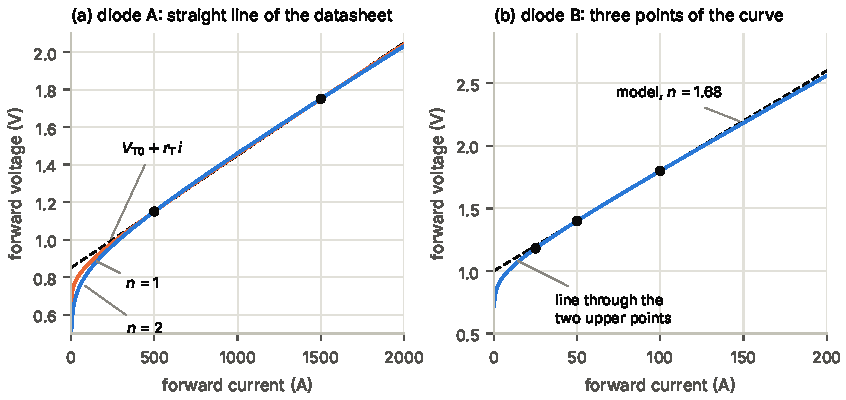
\includegraphics[width=\textwidth]{figures/fig_forward.pdf}
\caption{Forward characteristic of the model against the data. (a) Diode A: straight line of the datasheet (dashed), with its two points, and the secant fit for $n = 1$ and $n = 2$. (b) Diode B: fit through three points of the curve, and the straight line through the two upper points (dashed).}
\label{fig:forward}
\end{figure}

\subsection{Check in a simulated commutation cell}
\label{sec:cell}
The complete model, with the junction capacitance, the leakage and the series resistance, was simulated in the cell of Fig.~\ref{fig:model}b with $L = \VR/a$ and an RC snubber (Appendix~\ref{app:scripts}). The junction capacitances are estimates, $\Cjo = \SI{\lmACj}{\nano\farad}$ for A and \SI{\lmBCj}{\nano\farad} for B. Table~\ref{tab:cell} compares the simulation with the closed forms and Fig.~\ref{fig:cell} shows the waveforms.

\begin{table}[htb]
\centering\small
\caption{Simulated commutation cell against the closed forms. The closed forms are evaluated at the slope of the simulation; the charge is integrated down to \SI{\lmPEndPct}{\percent} of the peak, \eqref{eq:qrp}.}
\label{tab:cell}
\begin{tabular}{@{}lcc@{}}
\toprule
 & Diode A & Diode B \\
\midrule
Inductance $L = \VR/a$ & \SI{\lmAL}{\micro\henry} & \SI{\lmBL}{\micro\henry} \\
Snubber $\Rsn$, $\Csn$ & \SI{\lmARsn}{\ohm}, \SI{\lmACsn}{\nano\farad} & \SI{\lmBRsn}{\ohm}, \SI{\lmBCsn}{\nano\farad} \\
Slope at the current zero & \SI{\lmASimSlope}{\ampere\per\micro\second} ($\lmASimSlopeErr\,\%$) & \SI{\lmBSimSlope}{\ampere\per\micro\second} ($\lmBSimSlopeErr\,\%$) \\
\addlinespace
$\Irr$, closed form \eqref{eq:lambert} & \SI{\lmASimIrrCf}{\ampere} & \SI{\lmBSimIrrCf}{\ampere} \\
$\Irr$, simulation, diffusion current & \SI{\lmASimIrrDif}{\ampere} ($\lmASimIrrDifErr\,\%$) & \SI{\lmBSimIrrDif}{\ampere} ($\lmBSimIrrDifErr\,\%$) \\
$\Irr$, simulation, terminals & \SI{\lmASimIrrTerm}{\ampere} ($\lmASimIrrTermErr\,\%$) & \SI{\lmBSimIrrTerm}{\ampere} ($\lmBSimIrrTermErr\,\%$) \\
\addlinespace
$Q_\mathrm{r}$, closed form \eqref{eq:qrp} & \SI{\lmASimQCf}{\micro\coulomb} & \SI{\lmBSimQCf}{\micro\coulomb} \\
$Q_\mathrm{r}$, simulation, terminals & \SI{\lmASimQTerm}{\micro\coulomb} ($\lmASimQTermErr\,\%$) & \SI{\lmBSimQTerm}{\micro\coulomb} ($\lmBSimQTermErr\,\%$) \\
Charge of the junction capacitance, \eqref{eq:qc} & \SI{\lmAQc}{\micro\coulomb} & \SI{\lmBQc}{\micro\coulomb} \\
\addlinespace
$\trr$, straight line, closed form \eqref{eq:trr} & \SI{\lmASimTrrCf}{\micro\second} & \SI{\lmBSimTrrCf}{\nano\second} \\
$\trr$, straight line, simulation & \SI{\lmASimTrr}{\micro\second} & \SI{\lmBSimTrr}{\nano\second} \\
\addlinespace
Peak reverse voltage without snubber, \eqref{eq:vrm} & \SI{\lmAVpk}{\volt} & \SI{\lmBVpk}{\volt} \\
Peak reverse voltage, simulation with snubber & \SI{\lmASimVpk}{\volt} & \SI{\lmBSimVpk}{\volt} \\
Energy in the diode after the current zero & \SI{\lmASimEd}{\milli\joule} & \SI{\lmBSimEd}{\milli\joule} \\
Energy in the snubber resistor & \SI{\lmASimEr}{\milli\joule} & \SI{\lmBSimEr}{\milli\joule} \\
Sum & \SI{\lmASimEsum}{\milli\joule} & \SI{\lmBSimEsum}{\milli\joule} \\
Balance $\VR\Qrr + \Csn\VR^2/2$, \eqref{eq:ebal} & \SI{\lmASimEbal}{\milli\joule} & \SI{\lmBSimEbal}{\milli\joule} \\
\bottomrule
\end{tabular}
\end{table}

The table shows four things.
\begin{itemize}
\item The slope at the current zero is a little above $\VR/L$, because the forward voltage of the diode adds to $\VR$ while the current falls. The effect is below one percent here; it grows when $\VR$ is small.
\item The diffusion current of the simulation follows the closed form within \SI{0.5}{\percent}. The current at the terminals is higher at the peak, by \SI{0.1}{\percent} for A and \SI{1.5}{\percent} for B: this is the current of the junction capacitance while the voltage rises. For diode B the charge at the terminals exceeds the closed form by \SI{0.3}{\percent}, which is the charge of the junction capacitance, as the note of the standard says. For diode A that charge is negligible, and the \SI{0.1}{\percent} that remains comes from the slope, which is not exactly constant along the ramp because the forward voltage changes with the current.
\item The recovery time of the straight-line convention is reproduced within \SI{0.6}{\percent}.
\item The energy balance \eqref{eq:ebal} closes within \SI{0.5}{\percent}. For diode A the snubber is fast against the tail ($\Rsn\Csn = \SI{\lmARsnCsn}{\micro\second}$, $\taurr = \SI{\lmATrr}{\micro\second}$): it rounds the step of the voltage, but the peak is \SI{\lmASimVpk}{\volt}, practically the \SI{\lmAVpk}{\volt} that \eqref{eq:vrm} gives for the diode alone, and nearly all the energy stays in the diode. For diode B the snubber is as slow as the tail ($\Rsn\Csn = \SI{\lmBRsnCsn}{\nano\second}$, $\taurr = \SI{\lmBTrr}{\nano\second}$): it lowers the peak from \SI{\lmBVpk}{\volt} to \SI{\lmBSimVpk}{\volt} and takes more than half of the energy.
\end{itemize}

\begin{figure}[htb]
\centering
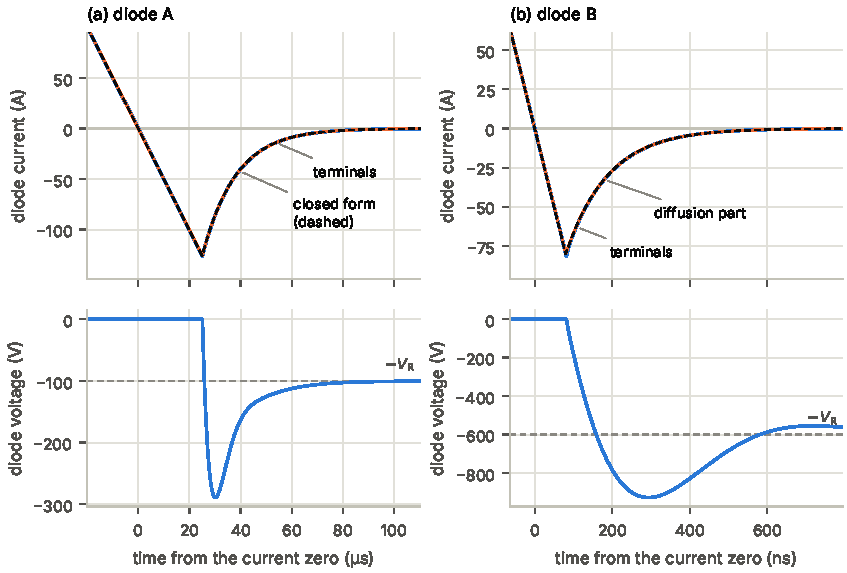
\includegraphics[width=\textwidth]{figures/fig_cell.pdf}
\caption{Simulated commutation cell with the snubber: current and voltage of the diode. The current at the terminals, the diffusion current and the closed form of Sec.~\ref{sec:ramp} (dashed) lie on each other; for diode B the terminal current is slightly above the diffusion current at the peak, by the current of the junction capacitance.}
\label{fig:cell}
\end{figure}

\subsection{Away from the datasheet point}
\label{sec:away}
Table~\ref{tab:awaya} and Fig.~\ref{fig:curves} show the two sets at other slopes and forward currents.

\begin{table}[htb]
\centering\small
\caption{Diode A away from the datasheet point, at $\IF = \SI{\lmAIf}{\ampere}$: the set of Table~\ref{tab:conv} against the assumed curve of the datasheet, and the set that the curve asks for at each slope (curve point converted with the softness of the datasheet point).}
\label{tab:awaya}
\begin{tabular}{@{}lccccc@{}}
\toprule
Slope $a$ [\si{\ampere\per\micro\second}] & \lmAAwayALo & \lmAAwayALoB & \lmAAwayARef & \lmAAwayAHiB & \lmAAwayAHi \\
\midrule
Length of the ramp, $x = \Tone/\tau$ & \lmAAwayXALo & \lmAAwayXALoB & \lmAAwayXARef & \lmAAwayXAHiB & \lmAAwayXAHi \\
$\Irr$ of the set [A] & \lmAAwayIrrALo & \lmAAwayIrrALoB & \lmAAwayIrrARef & \lmAAwayIrrAHiB & \lmAAwayIrrAHi \\
$\Qrr$ of the set [\si{\micro\coulomb}] & \lmAAwayQrrALo & \lmAAwayQrrALoB & \lmAAwayQrrARef & \lmAAwayQrrAHiB & \lmAAwayQrrAHi \\
$\Qrr$ of the datasheet curve [\si{\micro\coulomb}] & \lmAAwayDsALo & \lmAAwayDsALoB & \lmAAwayDsARef & \lmAAwayDsAHiB & \lmAAwayDsAHi \\
Set over curve & \lmAAwayRatioALo & \lmAAwayRatioALoB & \lmAAwayRatioARef & \lmAAwayRatioAHiB & \lmAAwayRatioAHi \\
\addlinespace
Curve point converted: $\tau$ [\si{\micro\second}] & \lmAAwayTauALo & \lmAAwayTauALoB & \lmAAwayTauARef & \lmAAwayTauAHiB & \lmAAwayTauAHi \\
Curve point converted: $\TM$ [\si{\micro\second}] & \lmAAwayTmALo & \lmAAwayTmALoB & \lmAAwayTmARef & \lmAAwayTmAHiB & \lmAAwayTmAHi \\
\bottomrule
\end{tabular}
\end{table}

For diode A the set is on a long ramp up to about \SI{10}{\ampere\per\micro\second}: its charge is proportional to the slope, while the curve of the datasheet grows with the exponent \num{\lmAQexp}. A decade below the datasheet point the set has a fifth of the charge of the curve. The last two rows are the sets that reproduce the curve at each slope: the lifetime goes from \SI{\lmAAwayTauALo}{\micro\second} at the lowest slope to \SI{\lmAAwayTauAHi}{\micro\second} at the highest, following \eqref{eq:taucurve} as long as the ramp is long. At the datasheet slope the forward current has almost no effect: \SI{\lmAAwayQrrFLo}{\micro\coulomb} at \SI{\lmAAwayFLo}{\ampere} and \SI{\lmAAwayQrrFHi}{\micro\coulomb} at \SI{\lmAAwayFHi}{\ampere}, against \SI{\lmAQrr}{\micro\coulomb} at \SI{\lmAIf}{\ampere}.

Diode B behaves in the opposite way. At twice the slope the charge grows from \SI{\lmBQrr}{\micro\coulomb} to \SI{\lmBAwayQrrAHi}{\micro\coulomb} only, and at half the slope it falls to \SI{\lmBAwayQrrALo}{\micro\coulomb}; at twice the forward current it is \SI{\lmBAwayQrrFHi}{\micro\coulomb} and at half the forward current \SI{\lmBAwayQrrFLo}{\micro\coulomb}. The peak current goes from \SI{\lmBAwayIrrALo}{\ampere} to \SI{\lmBAwayIrrAHi}{\ampere} over the two slopes and from \SI{\lmBAwayIrrFLo}{\ampere} to \SI{\lmBAwayIrrFHi}{\ampere} over the two currents. The point at half the slope and the point at twice the forward current have the same ratio $\IF/a$, and the second is twice the first, in the peak and in the charge: this is the homogeneity of Sec.~\ref{sec:exponents}.

\begin{figure}[htb]
\centering
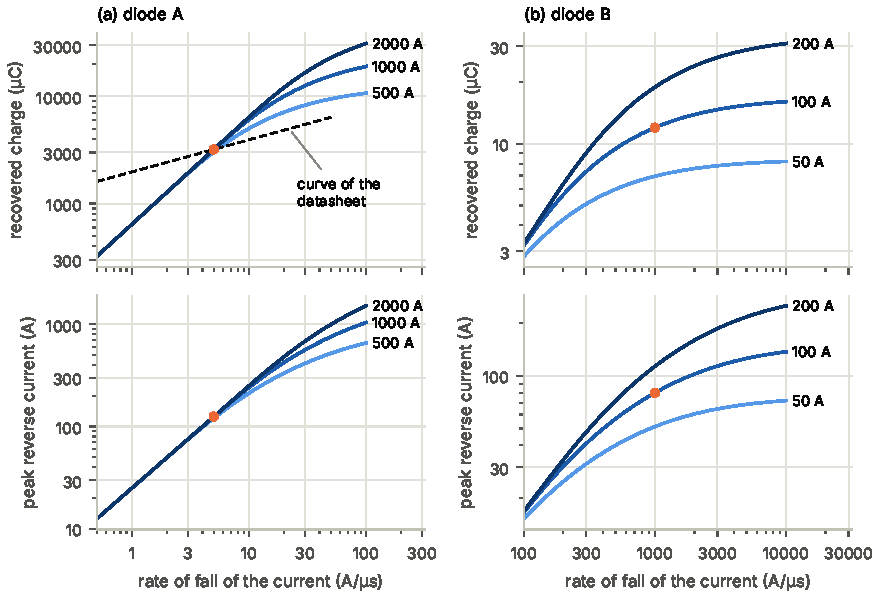
\includegraphics[width=\textwidth]{figures/fig_curves.pdf}
\caption{The two sets of Table~\ref{tab:conv} at other slopes, for half, one and twice the forward current of the datasheet test. The point is the datasheet point. For diode A the dashed line is the assumed curve of the datasheet.}
\label{fig:curves}
\end{figure}

\subsection{Temperature}
For diode B the datasheet gives the recovery at \SI{\lmBTtwo}{\celsius} as well. The same conversion gives $\taurr = \SI{\lmBTrrTtwo}{\nano\second}$, $\tau = \SI{\lmBTauTtwo}{\nano\second}$ and $\TM = \SI{\lmBTmTtwo}{\nano\second}$: against \SI{\lmBT}{\celsius} the lifetime is lower by \SI{\lmBTauTtwoPct}{\percent} and the transit time by \SI{\lmBTmTtwoPct}{\percent}. The two parameters do not scale together, so the softness changes with the temperature as well.

For diode A there are no data at a second temperature. As an example of the scaling \eqref{eq:scale}, a set with both time constants lower by \SI{\lmAIrrTtwoPct}{\percent} ($\tau = \SI{\lmATauTtwo}{\micro\second}$, $\TM = \SI{\lmATmTtwo}{\micro\second}$) gives at the datasheet slope $\Irr = \SI{\lmAIrrTtwo}{\ampere}$ and $\Qrr = \SI{\lmAQrrTtwo}{\micro\coulomb}$: the peak falls by the same \SI{\lmAIrrTtwoPct}{\percent} and the charge by \SI{\lmAQrrTtwoPct}{\percent}, because it goes with the square of the time constants. In the other direction, a charge known to be lower by \SI{\lmAQrrTtwoPct}{\percent} at a lower temperature asks for time constants lower by \SI{\lmAIrrTtwoPct}{\percent}.

\subsection{The same diodes in other descriptions}
\begin{table}[htb]
\centering\small
\caption{Quantities of the two sets in other conventions and test circuits.}
\label{tab:other}
\begin{tabular}{@{}llcc@{}}
\toprule
Quantity & & Diode A & Diode B \\
\midrule
$\trr$, straight line through \SI{90}{\percent} and \SI{25}{\percent} & \eqref{eq:trr} & \SI{\lmATrrLine}{\micro\second} & \SI{\lmBTrrLine}{\nano\second} \\
$\trr$, current at \SI{10}{\percent} of the peak & \eqref{eq:trr} & \SI{\lmATrrTen}{\micro\second} & \SI{\lmBTrrTen}{\nano\second} \\
$\trr$, triangle of equal charge, $2\Qrr/\Irr$ & & \SI{\lmATrrTri}{\micro\second} & \SI{\lmBTrrTri}{\nano\second} \\
Stretch factor $\trr\,a/\Irr$ (\SI{10}{\percent} convention) & & \lmAStretch & \lmBStretch \\
$\tb/\ta$, straight-line convention & & \lmASLine & \lmBSLine \\
\addlinespace
Abrupt commutation: $\Irr = \IF\tau/\TM$ & \eqref{eq:abrupt} & \SI{\lmAIrrFast}{\ampere} & \SI{\lmBIrrFast}{\ampere} \\
Abrupt commutation: $\Qrr = \IF(\tau-\taurr)$ & \eqref{eq:abrupt} & \SI{\lmAQrrFast}{\micro\coulomb} & \SI{\lmBQrrFast}{\micro\coulomb} \\
Static charge over datasheet charge, $\tau\IF/\Qrr$ & & \lmATauIfRatio & \lmBTauIfRatio \\
\addlinespace
Peak reverse voltage without snubber, $\VR(1+2/s)$ & \eqref{eq:vrm} & \SI{\lmAVpk}{\volt} & \SI{\lmBVpk}{\volt} \\
Recovery energy $\VR\,\Qrr$ & \eqref{eq:erec} & \SI{\lmAErec}{\milli\joule} & \SI{\lmBErec}{\milli\joule} \\
\bottomrule
\end{tabular}
\end{table}

Table~\ref{tab:other} gives the two sets in the other conventions of Sec.~\ref{sec:direct}. Two more test circuits complete the picture.

\emph{Resistive commutation of diode B.} With $\IF = \SI{\lmBStepIf}{\ampere}$ and $\IR = \SI{\lmBStepIr}{\ampere}$ the ratio $\IF/\IR = \lmBStepRatio$ is below $\TM/\tau = \lmBTmOverTau$: there is no storage phase. The reverse current starts from $\IF\tau/\TM = \SI{\lmBStepIzero}{\ampere}$ and falls to \SI{\lmBStepIrec}{\ampere} in \SI{\lmBStepTrr}{\nano\second}. With $\IF = \SI{\lmBStepIfTwo}{\ampere}$ the storage time \eqref{eq:ts} is \SI{\lmBStepTsTwo}{\nano\second} and the current reaches \SI{\lmBStepIrec}{\ampere} after \SI{\lmBStepTrrTwo}{\nano\second}. A recovery time measured in such a test has little to do with the \SI{\lmBTrrLine}{\nano\second} of the ramp test, and it depends on the two currents of the test.

\emph{Half-sine pulse on diode A.} A half sine of \SI{\lmASineLongMs}{\milli\second} with the slope of the datasheet at its zero has a peak of \SI{\lmASineLongIpk}{\kilo\ampere}; \eqref{eq:sine} gives a peak reverse current within $\lmASineLongErr\,\%$ of the long-ramp value $a(\tau-\taurr) = \SI{\lmALongIrr}{\ampere}$. With a half sine of \SI{\lmASineShortMs}{\milli\second} (peak \SI{\lmASineShortIpk}{\kilo\ampere}, $\omega\tau = \lmASineShortWt$) the difference is $\lmASineShortErr\,\%$. A half-sine test at line frequency and a ramp test with the same slope at the zero are the same test for the model.

\subsection{Sensitivity of the two conversions}
\begin{table}[htb]
\centering\small
\caption{Relative change of the parameters of the exact conversion for a relative change of one datum of one percent (numerical derivatives of \eqref{eq:taurr}, \eqref{eq:iter} and \eqref{eq:tm}).}
\label{tab:sensex}
\begin{tabular}{@{}lcccccc@{}}
\toprule
 & \multicolumn{3}{c}{Diode A} & \multicolumn{3}{c}{Diode B} \\
\cmidrule(lr){2-4}\cmidrule(l){5-7}
Datum & $\tau$ & $\taurr$ & $\TM$ & $\tau$ & $\taurr$ & $\TM$ \\
\midrule
$\Qrr$ & $\lmASensTauQ$ & $\lmASensTrrQ$ & $\lmASensTmQ$ & $\lmBSensTauQ$ & $\lmBSensTrrQ$ & $\lmBSensTmQ$ \\
$\Irr$ & $\lmASensTauI$ & $\lmASensTrrI$ & $\lmASensTmI$ & $\lmBSensTauI$ & $\lmBSensTrrI$ & $\lmBSensTmI$ \\
$a$ & $\lmASensTauA$ & $\lmASensTrrA$ & $\lmASensTmA$ & $\lmBSensTauA$ & $\lmBSensTrrA$ & $\lmBSensTmA$ \\
$\IF$ & $\lmASensTauF$ & $\lmASensTrrF$ & $\lmASensTmF$ & $\lmBSensTauF$ & $\lmBSensTrrF$ & $\lmBSensTmF$ \\
\bottomrule
\end{tabular}
\end{table}
For diode A the numbers of Table~\ref{tab:sensex} are those of \eqref{eq:sens} with $s = \lmAS$ within \num{0.01}, and the forward current has no weight. A peak current higher by \SI{5}{\percent} at the same charge moves $\tau$ by $\lmAFiveTau\,\%$, $\taurr$ by $\lmAFiveTrr\,\%$ and $\TM$ by $\lmAFiveTm\,\%$. For diode B the same change gives $\lmBFiveTau\,\%$, $\lmBFiveTrr\,\%$ and $\lmBFiveTm\,\%$. On its short ramp the lifetime depends on the forward current of the test almost as much as on the peak current, and hardly on the slope: the forward current of the datasheet test has to be known and used.

%=====================================================================
\section{Procedure}
\label{sec:procedure}
\begin{enumerate}
\item \emph{Choose the data.} Take $\Irr$ and $\Qrr$ at the temperature of interest and at the slope nearest to that of the application, with the forward current, the slope and the reverse voltage of the test. Note whether they are maximum or typical values and which convention defines the recovery time, if it is used (Table~\ref{tab:kappa}).
\item \emph{Check the pair.} The charge has to exceed the triangle: $\Qrr > \Irr^2/(2a)$. Compute $\Irr/\IF$: below \num{0.1} the ramp of the test is long; above, it may not be (Table~\ref{tab:valid}).
\item \emph{Tail time constant.} $\taurr = \Qrr/\Irr - \Irr/(2a)$, \eqref{eq:taurr}; from other pairs, \eqref{eq:fromtrr} to \eqref{eq:fromq}.
\item \emph{Lifetime.} Iterate \eqref{eq:iter} from $\tau = \taurr + \Irr/a$. On a long ramp the starting value is the result.
\item \emph{Transit time.} $\TM = \tau\taurr/(\tau-\taurr)$, \eqref{eq:tm}. The softness of the diode on a long ramp is $2\TM/\tau$.
\item \emph{Conduction.} Choose $n$ (2 for a power diode in high injection) and fit $\IS$ and $\RS$ to the straight line, \eqref{eq:tangent} or \eqref{eq:secant}, or fit all three to points of the curve, \eqref{eq:points}. Multiply $\IS$ by $(\tau+\TM)/\tau$ if the implementation writes the junction law with $\tau\,\IS^{*}$.
\item \emph{Blocking.} $\Rr$ from the reverse current at the working voltage and temperature; $\Cjo$ from the datasheet or from an estimate, \eqref{eq:cj}.
\item \emph{Verify.} Put the set on the test ramp, with \eqref{eq:lambert} or with a simulation of the test cell, and compare $\Irr$, $\Qrr$ and $\trr$ with the datasheet. Then look at the working point of the application: slope, forward current and length of the ramp in lifetimes. If the slope is far from that of the data, convert again from the nearest point of the datasheet curve (Sec.~\ref{sec:slope}).
\item \emph{Bracket.} Where the result depends on the softness (peak voltage, damping) or on the spread between devices, repeat with $\TM$ at the ends of its range (Sec.~\ref{sec:sens}) and with the scaled set \eqref{eq:scale}.
\end{enumerate}

%=====================================================================
\appendix
\section{Where the two charges come from}
\label{app:lumped}
This appendix gives a short derivation of the equations of the model, to show what the two charges and the transit time stand for. It follows the lumped-charge idea of \cite{linvill1958} that \cite{lauritzen1991} applies to the diode; the choice of the profile below is one way to do it, not a quotation of the paper.

\subsection*{Charge-control equation}
Take the lightly doped base of a p\textsuperscript{+}--n\textsuperscript{--}--n\textsuperscript{+} diode, of width $2d$ and area $A$, in high injection: electrons and holes have the same concentration $p(x,t)$, which obeys the ambipolar diffusion equation
\begin{equation}
\frac{\partial p}{\partial t} = D\,\frac{\partial^2 p}{\partial x^2} - \frac{p}{\tau} , \qquad -d \leq x \leq d ,
\label{eq:diffusion}
\end{equation}
with the ambipolar diffusion constant $D$ and the high-injection lifetime $\tau$. With ideal emitters the current enters as a gradient of the concentration at the two edges; for equal mobilities of electrons and holes, $i = 2qAD\,\partial p/\partial x$ at $x = d$ and the opposite gradient at $x = -d$. Integrating \eqref{eq:diffusion} over the base, with the stored charge $Q = qA\int p\,\diff x$, gives
\begin{equation}
\frac{\diff Q}{\diff t} = i - \frac{Q}{\tau} .
\label{eq:cc}
\end{equation}
This is the charge-control equation, and it is exact. It is \eqref{eq:qm} if the middle charge is the whole stored charge, $\qM = Q$. What it does not say is how the current depends on the state of the base: for that the shape of the profile is needed.

\subsection*{Two lumps}
Describe the profile with two numbers, the concentration $p_\mathrm{E}$ at the edges and $p_\mathrm{M}$ in the middle, joined by a parabola: $p(x) = p_\mathrm{M} + (p_\mathrm{E}-p_\mathrm{M})\,(x/d)^2$. Then the gradient at the edge is $2\,(p_\mathrm{E}-p_\mathrm{M})/d$ and the stored charge is $Q = \tfrac{2}{3}\,qAd\,(2p_\mathrm{M}+p_\mathrm{E})$. Define the edge charge as the charge the base would hold if the edge concentration filled it, $\qE = 2qAd\,p_\mathrm{E}$. Then $\qE - \qM = \tfrac43\,qAd\,(p_\mathrm{E}-p_\mathrm{M})$ and the current is
\begin{equation}
i = \frac{4qAD\,(p_\mathrm{E}-p_\mathrm{M})}{d} = \frac{\qE-\qM}{\TM} , \qquad \TM = \frac{d^2}{3D} .
\label{eq:tmgeom}
\end{equation}
This is \eqref{eq:idif}: the current is the diffusion from the edges to the middle, and the transit time is the diffusion time over the half width of the base.

\subsection*{Junction law}
In high injection the product of the carrier concentrations at the two edges of the base follows the sum $\vj$ of the two junction voltages, $p_\mathrm{E}^2 = n_\mathrm{i}^2\,e^{\vj/\VT}$ for a symmetric profile, so $p_\mathrm{E} = n_\mathrm{i}\,e^{\vj/(2\VT)}$: the edge charge follows the junction voltage with the emission coefficient $n = 2$. This is \eqref{eq:qe}. A reverse voltage brings the edge concentration to zero and can do no more: this is the blocked junction, $\qE = 0$, of Sec.~\ref{sec:regimes}.

\subsection*{How well one number can do}
The transit time of \eqref{eq:tmgeom} comes from one profile, and other states of the base ask for other values. In the steady state the exact profile of \eqref{eq:diffusion} is a hyperbolic cosine, and the ratio of the edge charge to the stored charge gives
\begin{equation}
\frac{\TM}{\tau} = \frac{d}{L}\,\coth\frac{d}{L} - 1 , \qquad L = \sqrt{D\,\tau} ,
\label{eq:tmstatic}
\end{equation}
which is $d^2/(3D\tau)$ for a base narrower than the diffusion length $L$, the value of \eqref{eq:tmgeom}. After blocking, with the concentration held at zero at both edges, the slowest mode of \eqref{eq:diffusion} is a cosine that decays with the rate $1/\tau + \pi^2 D/(4d^2)$; compared with $1/\taurr = 1/\tau + 1/\TM$ it asks for $\TM = 4d^2/(\pi^2 D)$, which is \SI{22}{\percent} above \eqref{eq:tmgeom}. So the transit time is of the order of $d^2/(3D)$, but it is not a constant that could be computed from the geometry: it is an effective parameter, to be taken from the recovery waveform.

The order of magnitude is still a useful check of a conversion. With an ambipolar diffusion constant of \SI{\lmADcm}{\centi\metre\squared\per\second}, a rough value for silicon at \SI{\lmAT}{\celsius} [M] \cite{lutz}, the transit time of diode A corresponds to a base width $2d$ of \SI{\lmAWpar}{\micro\metre} with \eqref{eq:tmgeom}, \SI{\lmAWmode}{\micro\metre} with the slowest mode and \SI{\lmAWstat}{\micro\metre} with \eqref{eq:tmstatic}; the diffusion length is \SI{\lmALdiff}{\micro\metre}. About half a millimetre is a plausible base for a diode of \SI{\lmAVrrmKv}{\kilo\volt} [M]. For diode B, with \SI{\lmBDcm}{\centi\metre\squared\per\second}, the same three relations give \SI{\lmBWpar}{\micro\metre}, \SI{\lmBWmode}{\micro\metre} and \SI{\lmBWstat}{\micro\metre}. The data of both diodes are assumed, so these numbers say nothing about real parts; they show how the check reads. On a real datasheet a width far from what the voltage class suggests means that the two parameters are behavioural: they reproduce the test waveform, not the inside of the device. To some degree this is always so, because a real base is not symmetric: electrons and holes have different mobilities, and the charge is removed first at the p\textsuperscript{+} side.

%=====================================================================
\section{Proofs}
\label{app:proofs}
\subsection{Closed form of the peak}
\label{app:lambert}
Write the first of \eqref{eq:norm} as $y = c - c\,e^{-\lambda}e^{-y}$ with $c = 1-\rho$, and put $w = y - c$. Then $w = -c\,e^{-(\lambda+c)}\,e^{-w}$, that is
\begin{equation}
w\,e^{w} = -c\,e^{-(\lambda+c)} .
\end{equation}
The right-hand side lies between $-1/e$ and zero, because $c\,e^{-c} \leq 1/e$. Since $0 < y < c < 1$, $w$ lies between $-1$ and zero, which is the range of the principal branch: $w = W_0(-c\,e^{-(\lambda+c)})$, and \eqref{eq:lambert} follows.

\subsection{Convergence of the iteration}
\label{app:contraction}
Let $g(\tau) = \taurr + \ta/(1-e^{-\Tone/\tau})$ be the right-hand side of \eqref{eq:iter}, for $\tau > 0$. With $x = \Tone/\tau$ its derivative is
\begin{equation}
g'(\tau) = \frac{\ta}{\Tone}\,\frac{x^2\,e^{-x}}{(1-e^{-x})^2} = \frac{\ta}{\Tone}\left(\frac{x/2}{\sinh(x/2)}\right)^{2} .
\end{equation}
The bracket lies between zero and one, so
\begin{equation}
0 < g'(\tau) < \frac{\ta}{\Tone} = \frac{\Irr}{\IF+\Irr} < 1 .
\end{equation}
The map $g$ is a contraction on the whole half line: it has one fixed point, the iteration converges to it from any starting value, and the error shrinks at each step by a factor smaller than $\Irr/(\IF+\Irr)$. Since $g$ is increasing and $g(\taurr+\ta) > \taurr+\ta$, the sequence that starts from the closed form rises monotonically to the solution: the closed form always underestimates the lifetime. On a long ramp the bracket is very small and two or three steps are enough; when $\Irr$ is close to $\IF$ and the ramp is short the factor is close to one half. The solution exists for every $\taurr > 0$, so the only condition on the data is $\Qrr > \Irr^2/(2a)$. The transit time \eqref{eq:tm} is positive because the solution has $\tau > \taurr + \ta$.

\subsection{Exponents}
\label{app:exponents}
Differentiating the first of \eqref{eq:norm} with respect to $\lambda$, with $(1-\rho)\,e^{-(\lambda+y)} = 1-\rho-y$, gives
\begin{equation}
\frac{\diff y}{\diff\lambda} = \frac{1-\rho-y}{\rho+y} .
\end{equation}
With $\Irr = a\tau\,y(\lambda)$ and $\lambda = \IF/(a\tau)$, $\partial\ln\Irr/\partial\ln a = 1 - (\lambda/y)\,\diff y/\diff\lambda$, which is the first of \eqref{eq:exponents}; the second follows in the same way from $\Qrr = a\tau^2\,(y^2/2+\rho y)$. The derivatives with respect to $\ln\IF$ are $(\lambda/y)\,\diff y/\diff\lambda$ and its counterpart for the charge, so the sums are one, \eqref{eq:euler}.

%=====================================================================
\section{Scripts}
\label{app:scripts}
Two Python files sit next to this note. They need NumPy, SciPy and Matplotlib only.
\begin{itemize}
\emergencystretch=3em
\item \texttt{lm\_conversion.py} is a module with the relations of the note in SI units: the ramp solution (\texttt{ramp\_recovery}, \texttt{ramp\_peak\_norm}, \texttt{ramp\_exponents}, \texttt{ramp\_waveform}), the conventions of the recovery time (\texttt{trr\_factor}), the other test circuits (\texttt{step\_recovery}, \texttt{sine\_peak}), the conversions (\texttt{lm\_from\_irr\_qrr}, \texttt{lm\_from\_irr\_trr}, \texttt{irr\_from\_qrr\_trr}, \texttt{irr\_from\_qrr\_softness}, \texttt{sensitivities}), the forward fits (\texttt{forward\_tangent}, \texttt{forward\_secant}, \texttt{forward\_points}), the junction capacitance, and the simulation of the commutation cell with the tools to read a waveform as a datasheet would (\texttt{simulate\_cell}, \texttt{measure}). Run as a program it tests the closed forms against a step-by-step integration.
\item \texttt{lm\_conversion\_calc.py} holds the data of the two diodes at its top and produces the numbers and the figures of the note: the log \texttt{lm\_conversion\_results.txt}, the file \texttt{lm\_conversion\_values.tex} with every number quoted here as a macro, and \texttt{figures/*.pdf}. It runs in a few seconds. To convert another diode, replace the data of one of the two dictionaries.
\end{itemize}

\emph{Commutation cell.} The cell of Fig.~\ref{fig:model}b has four states: the current $i_\mathrm{sw}$ of the switch, the middle charge, the junction voltage and the voltage $v_\mathrm{c}$ of the snubber capacitor,
\begin{equation}
\begin{aligned}
L\,\frac{\diff i_\mathrm{sw}}{\diff t} &= \VR + v , &\qquad \frac{\diff\qM}{\diff t} &= \frac{\qE-\qM}{\TM} - \frac{\qM}{\tau} , \\
\Cj(\vj)\,\frac{\diff\vj}{\diff t} &= i - \frac{\qE-\qM}{\TM} - \frac{\vj}{\Rr} , &\qquad \Csn\,\frac{\diff v_\mathrm{c}}{\diff t} &= \frac{v - v_\mathrm{c}}{\Rsn} ,
\end{aligned}
\end{equation}
with $i = \IF - i_\mathrm{sw} - (v-v_\mathrm{c})/\Rsn$, $v = \vj + \RS\,i$ and $\qE$ from \eqref{eq:qe}. The system is stiff, because the junction voltage reacts much faster than the charge; it is integrated with an implicit method (Radau, relative tolerance $10^{-9}$) and the analytical Jacobian. The waveform is then read as in a test: slope just before the current zero, peak, charge down to \SI{\lmPEndPct}{\percent} of the peak, recovery time by the straight line.

%=====================================================================
\begin{thebibliography}{99}
\small
\item[] References marked [M] are quoted from memory: their bibliographic data, and the statements taken from them, have to be checked on the source before use in a design document. The others were read, or their bibliographic data verified, when the note was written; the documentation of the simulators was read on the web in November 2026.

\bibitem{lauritzen1991}
P.~O.~Lauritzen, C.~L.~Ma, ``A simple diode model with reverse recovery'', \emph{IEEE Trans. Power Electron.}, vol.~6, no.~2, pp.~188--191, Apr.~1991. doi:\,10.1109/63.76804.

\bibitem{ma1993}
C.~L.~Ma, P.~O.~Lauritzen, ``A simple power diode model with forward and reverse recovery'', \emph{IEEE Trans. Power Electron.}, vol.~8, no.~4, pp.~342--346, Oct.~1993. doi:\,10.1109/63.261002.

\bibitem{linvill1958}
J.~G.~Linvill, ``Lumped models of transistors and diodes'', \emph{Proc. IRE}, vol.~46, no.~6, pp.~1141--1152, June~1958. doi:\,10.1109/JRPROC.1958.286896.

\bibitem{pemodels}
University of Washington, Department of Electrical Engineering, web pages on power semiconductor device models: \emph{Basic Diode with Reverse Recovery}, updated 23~January 2013, \url{https://labs.ece.uw.edu/pemodels/modtext/diode-b.html}, and the page of the diode with forward and reverse recovery, \url{https://labs.ece.uw.edu/pemodels/modtext/diode-fr.html}.

\bibitem{iec60747}
IEC~60747-2:2025, \emph{Semiconductor devices -- Part~2: Discrete devices -- Rectifier diodes}, Ed.~4.0, September 2025. Definitions 3.3.10 (peak reverse recovery current), 3.5.2 (reverse recovery time), 3.5.3 and 3.5.4 (rise and fall time), 3.5.5 (recovered charge) were read in the public preview of the standard. Clause 6.3.5 (measuring methods) is quoted from the table of contents; the definitions of the threshold voltage and of the slope resistance were not read.

\bibitem{an6481}
Dynex Semiconductor, \emph{RC Snubber Design for Dynex Thyristors and Diodes}, Application Note AN6481-1, LN43754, November 2024. Sec.~2.1 (reverse recovery waveform, recovery time by the straight line through \SI{90}{\percent} and \SI{25}{\percent} of the peak, softness), Sec.~2.2, Eqs.~(1) and~(2) (exponential tail and its time constant).

\bibitem{an5028}
STMicroelectronics, \emph{Calculation of turn-off power losses generated by an ultrafast diode}, Application Note AN5028, Rev.~1, October 2017. Definitions of the recovery time, of the fraction $k$ and of the softness.

\bibitem{an5950}
D.~Chamund, C.~Rout, \emph{Understanding i\textsuperscript{2} Phase Control Thyristor Datasheets}, Dynex Semiconductor, Application Note AN5950-1, LN26885, September 2009. Figs.~12 and~13 (stored charge and reverse current against the slope).

\bibitem{mathworks}
MathWorks, Simscape Electrical documentation, reference page of the block \emph{Diode}, release R2026b, sections ``Charge Dynamics'', ``How the Block Calculates TM and tau'' and ``Alternatives to Specifying trr Directly''. \url{https://www.mathworks.com/help/sps/ref/diode.html}.

\bibitem{plecs}
Plexim, PLECS documentation, version 5.0, component \emph{Diode with Reverse Recovery}. \url{https://docs.plexim.com/plecs/5.0/components-by-category/rrdiode/}.

\bibitem{schlangenotto1969}
H.~Schlangenotto, W.~Gerlach, ``On the effective carrier lifetime in p-s-n rectifiers at high injection levels'', \emph{Solid-State Electronics}, vol.~12, no.~4, pp.~267--275, 1969. doi:\,10.1016/0038-1101(69)90008-2.

\bibitem{nagel1975}
[M] L.~W.~Nagel, \emph{SPICE2: A computer program to simulate semiconductor circuits}, Memorandum ERL-M520, University of California, Berkeley, 1975. Diode model with the transit time \texttt{TT}.

\bibitem{lutz}
[M] J.~Lutz, H.~Schlangenotto, U.~Scheuermann, R.~De~Doncker, \emph{Semiconductor Power Devices: Physics, Characteristics, Reliability}, Springer, 2011. Carrier lifetime, ambipolar diffusion, reverse recovery, reverse current.

\end{thebibliography}

\end{document}
